%!TEX program = lualatex
%----------------------------------------------------------------------------------------
%    PACKAGES AND THEMES
%----------------------------------------------------------------------------------------

\documentclass[aspectratio=169,xcolor=dvipsnames]{beamer}
\usetheme{SimplePlus}

\usepackage{hyperref}
\usepackage{graphicx} % Allows including images
\usepackage{booktabs} % Allows the use of \toprule, \midrule and \bottomrule in tables
\usepackage[german]{babel}

\usepackage{tikz}
\usepackage[compat=1.1.0]{tikz-feynman}
%\usepackage[table]{xcolor}
\usepackage{emoji}

\renewcommand{\arraystretch}{1.5}

%----------------------------------------------------------------------------------------
%    TITLE PAGE
%----------------------------------------------------------------------------------------

\title{Grundlagen Teilchenphysik}
\subtitle{}

\author{Anna von Karstedt, Hannes Richardt}

\institute
{
    Fakultät für Mathematik, Informatik und Naturwissenschaften \\
    Universität Hamburg % Your institution for the title page
}
\date{\today} % Date, can be changed to a custom date

%----------------------------------------------------------------------------------------
%    PRESENTATION SLIDES
%----------------------------------------------------------------------------------------

\begin{document}


\begin{frame}
    % Print the title page as the first slide
    \titlepage
\end{frame}

\begin{frame}{Gliederung}
    % Throughout your presentation, if you choose to use \section{} and \subsection{} commands, these will automatically be printed on this slide as an overview of your presentation
    \tableofcontents
\end{frame}

\section{Standardmodell}
\subsection{Fermionen}

\begin{frame}{Woraus besteht Materie?}
    \begin{tikzpicture}
        % draw a horizontal line
        \draw (0,0) -- (14,0);
        % draw vertical lines
        \foreach \x in {1,3,5,7,9,11,13}
        \draw (\x cm,3pt) -- (\x cm,-4pt);
        % draw nodes to add events
        \draw (1,0) node[below=3pt] {400 v.Chr.} node[above=25pt] {4 Elemente};
        \draw (3,0) node[above=3pt] {400 v.Chr.} node[below=25pt] {Begriff des Atoms};
        \draw (5,0) node[below=3pt] {1897} node[above=25pt] {Entdeckung Elektron};
        \draw (7,0) node[above=3pt]{1919} node[below=25pt] {Rosinenkuchenmodell};
        \draw (9,0) node[below=3pt] {1936} node[above=25pt] {Entdeckung Myon};
        \draw (11,0) node[above=3pt] {1960er} node[below=25pt] {Quarks};
        \draw (13,0) node[below=3pt] {2012} node[above=25pt] {Higgs-Teilchen};

    \end{tikzpicture}
\end{frame}

\begin{frame}{Elementarteilchen}
    \begin{columns}[c]
        \column{.45\textwidth}
        \begin{itemize}
            \item Teilchenzoo
            \item Standartmodell der Teilchen
            \item kleinsten unteilbaren Bestandteile von Materie
            \item Fermionen und Bosonen
            \item Durchmesser Null
        \end{itemize}
        \column{.45\textwidth}
        \begin{figure}
            \centering
            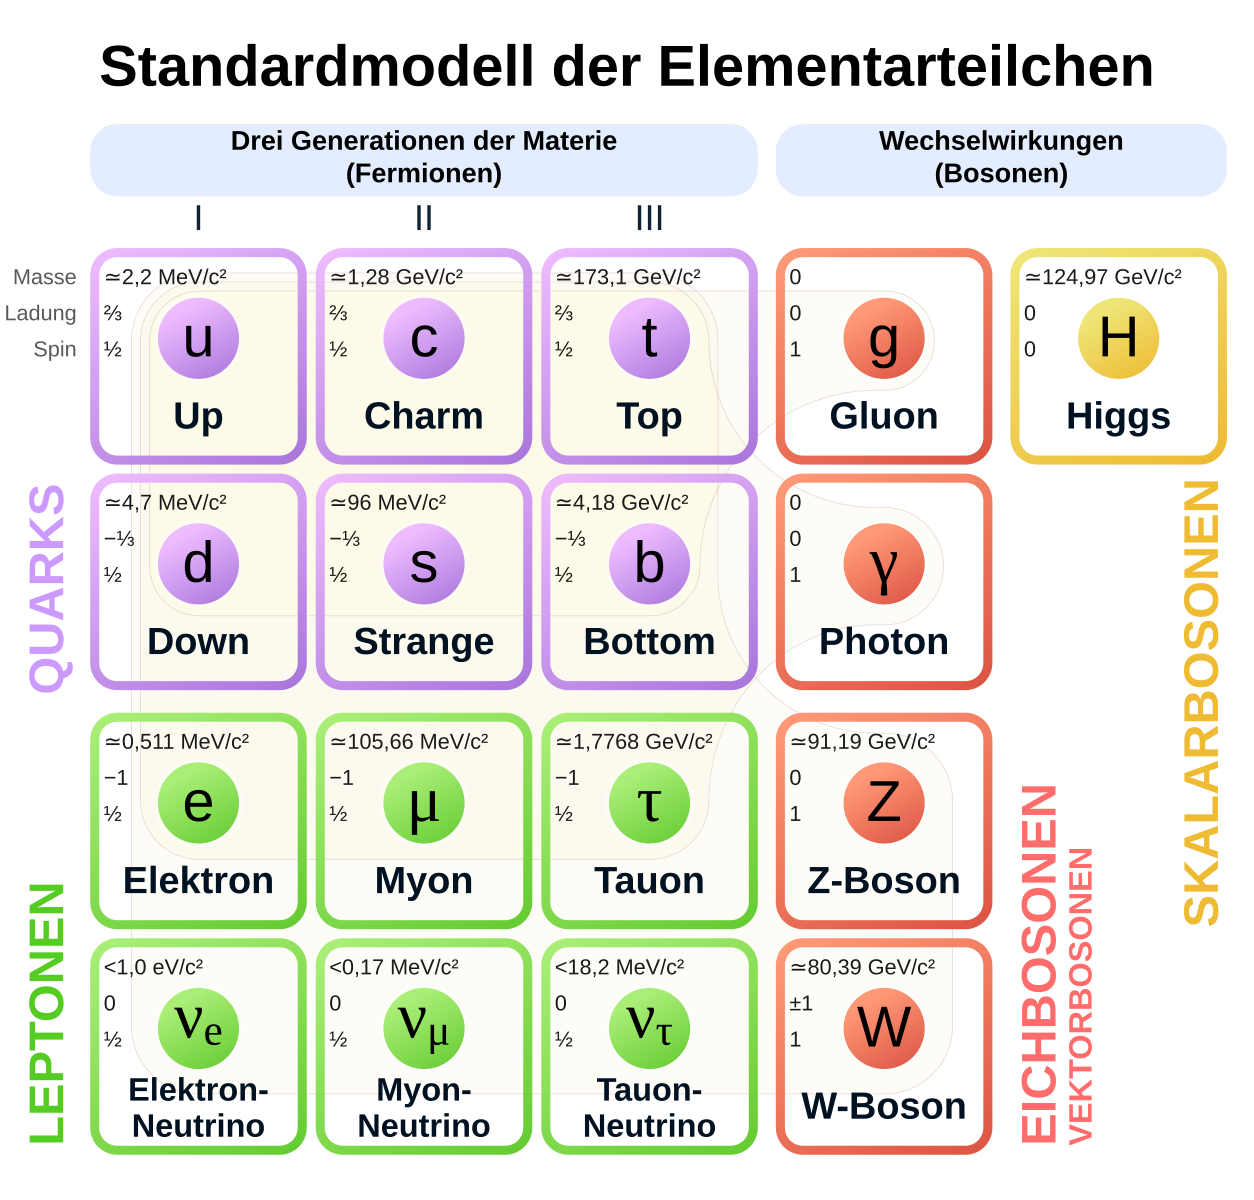
\includegraphics[width=0.9\linewidth]{figures/standartmodell.png}
            \caption{Standardmodell}
            \label{fig:standardmodell}
        \end{figure}
    \end{columns}
\end{frame}
\begin{frame}{Durchmesser Null}
    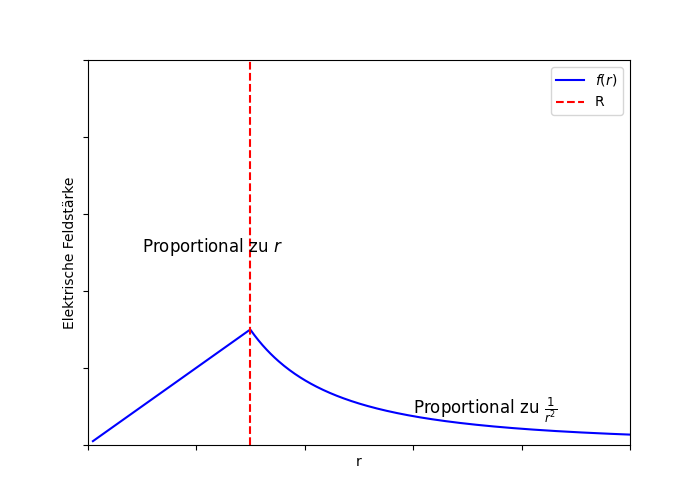
\includegraphics[width=10cm]{figures/elektron.png}
\end{frame}
\begin{frame}{Fermionen}
    \begin{columns}[c]
        \column{.45\textwidth}
        \begin{itemize}
            \item Grundlage der Materie
            \item halbzahliger Spin
            \item magnetische Spinquantenzahl
            \item Helizität
            \item Masse
            \item Ladung
            \item Zustandsvektor $|\psi_1\rangle$
            \item Pauliprinzip
        \end{itemize}
        \column{.45\textwidth}
        \begin{exampleblock}{Antisymmetrische Wellenfunktion}
            $|\Psi\rangle = \frac{1}{\sqrt{2}} \left( |\psi_1\rangle \otimes |\psi_2\rangle - |\psi_2\rangle \otimes |\psi_1\rangle \right)$\\
            $ $\\
            Wenn: $|\psi_1\rangle = |\psi_2\rangle$\\
            $ $\\
            $\Rightarrow |\Psi\rangle = 0$
        \end{exampleblock}
    \end{columns}
\end{frame}
\begin{frame}{Quarks}
    \begin{columns}[c]
        \column{.2\textwidth}
        \begin{figure}
            \centering
            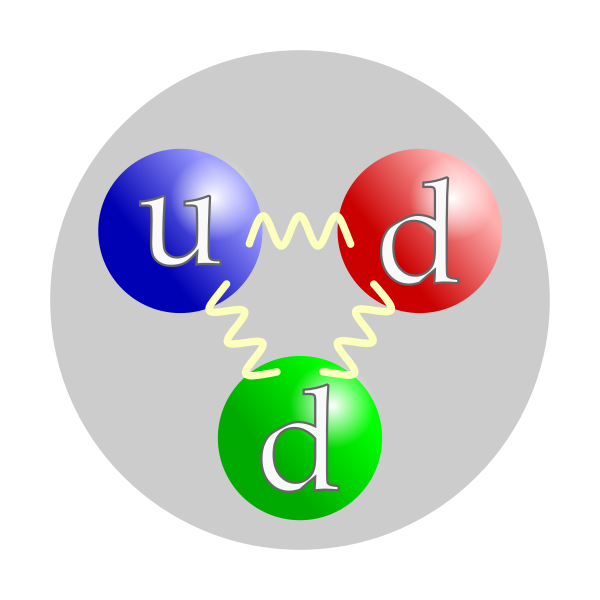
\includegraphics[width=0.5\linewidth]{figures/Neutron.png}
            \caption{Neutron}
            \label{fig:Neutron}
        \end{figure}
        \begin{figure}
            \centering
            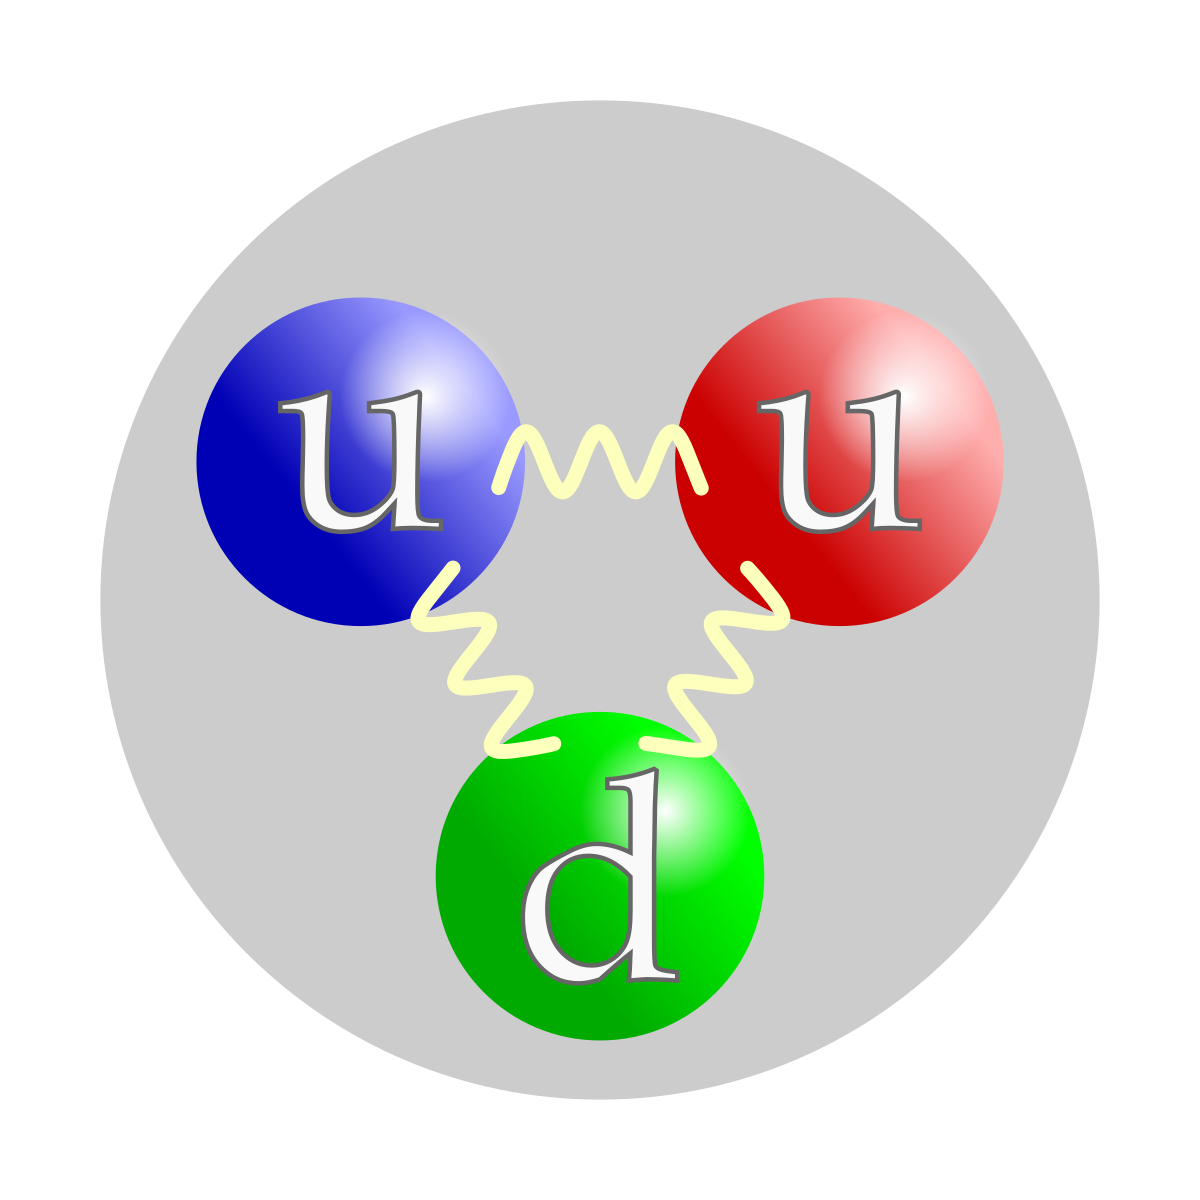
\includegraphics[width=0.5\linewidth]{figures/proton.png}
            \caption{Proton}
            \label{fig:proton}
        \end{figure}
        \column{.8\textwidth}
        \vspace{5pt}
        \begin{table}
            \centering
            \begin{tabular}{c|c|c|c}
                             & 1. Generation  & 2. Generation   & 3.Generation    \\ \hline
                             & \bf Up         & \bf Charm       & \bf Top         \\ \hline
                Ladung in e  & $+\frac{2}{3}$ & $+\frac{2}{3}$  & $+\frac{2}{3}$  \\ \hline
                Masse in MeV & $2,16\pm 0,07$ & $1273,0\pm 4,6$ & $172570\pm 290$ \\ \hline

                             & \bf Down       & \bf Strange     & \bf Bottom      \\ \hline
                Ladung in e  & $-\frac{1}{3}$ & $-\frac{1}{3}$  & $-\frac{1}{3}$  \\ \hline
                Masse in MeV & $4,7\pm 0,07$  & $93,5\pm0,8$    & $4183\pm 290$   \\
            \end{tabular}
            \caption{Quarks}
            \label{tab:quarks}
        \end{table}
    \end{columns}

\end{frame}
\begin{frame}{Baryonen}
    \begin{columns}[c]
        \column{.45\textwidth}
        \begin{itemize}
            \item 3 Quarks
        \end{itemize}
        \begin{block}{Baryonenzahl}
            Jedem Baryonen wird die Baryonenzahl 1 und jedem Antibaryonen die Zahl -1 zugeordnet
        \end{block}
        \begin{itemize}
            \item Erhaltungsprinzip
            \item Bsp. $ n \rightarrow p+e^- +av_e$
        \end{itemize}

        \column{.45\textwidth}
        \begin{figure}
            \centering
            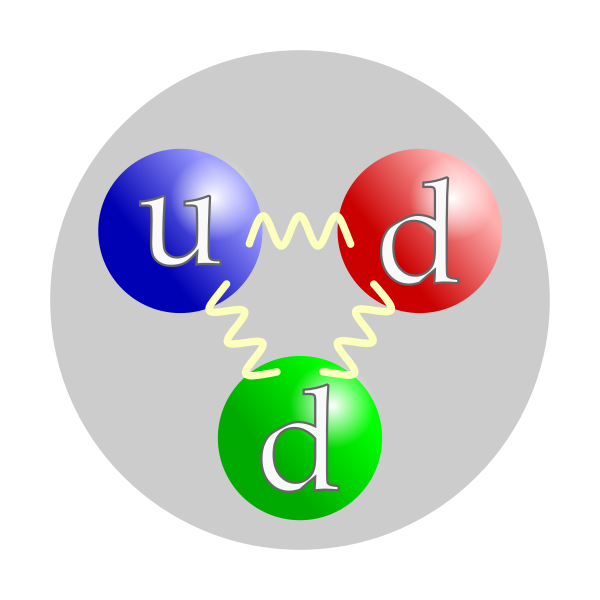
\includegraphics[width=0.45\linewidth]{figures/Neutron.png}
            \caption{Neutron}
            \label{fig:neutron}
        \end{figure}
    \end{columns}
\end{frame}
\begin{frame}{Leptonen}
    \begin{tabular}{c|c|c|c}
        \centering
                     & 1. Generation         & 2. Generation     & 3.Generation       \\ \hline
                     & \bf Elektron          & \bf Myon          & \bf Tauon          \\ \hline
        Ladung in e  & $-1$                  & $-1$              & $-1$               \\ \hline
        Masse in MeV & $0,511$               & $105,66$          & $1777$             \\ \hline

        Lebensdauer  & stabil                & $2,197*10^{-6}$   & $2,9*10^{-13}$     \\ \hline
                     & \bf Elektron-Neutrino & \bf Myon-Neutrino & \bf Tauon-Neutrino \\ \hline
        Ladung in e  & $0$                   & $0$               & $0$                \\ \hline
        Masse in MeV & $<9*10^{-7}$          & $<0,17$           & $<15,5$            \\ \hline
        Lebensdauer  & stabil                & stabil            & stabil
    \end{tabular}
\end{frame}


\begin{frame}{Myonen}
    \begin{columns}[c]
        \column{.45\textwidth}
        \begin{itemize}
            \item 200 mal größere Masse als ein Elektron
            \item entstehen bei Höhenstrahlung
            \item instabil Lebensdauer 2,2 Mikrosekunden
            \item spezielle Relativitätstheorie
        \end{itemize}
        \column{.4\textwidth}
        \begin{figure}
            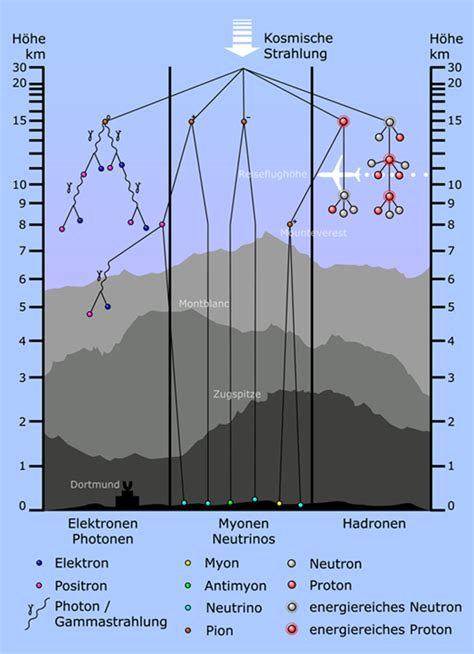
\includegraphics[width=0.7\linewidth]{figures/th.jpg}
            \caption{Höhenstrahlung}
            \label{fig:th}
        \end{figure}
    \end{columns}
\end{frame}
\begin{frame}{Neutrino}
    \begin{columns}[c]
        \column{.45\textwidth}
        \begin{itemize}
            \item Antwort auf die fehlende Energie beim Betazerfall
            \item ungeladen und sehr leicht
            \item kaum Reaktion
            \item werden von Sternen abgestrahlt
        \end{itemize}
        \column{.4\textwidth}
        \begin{figure}
            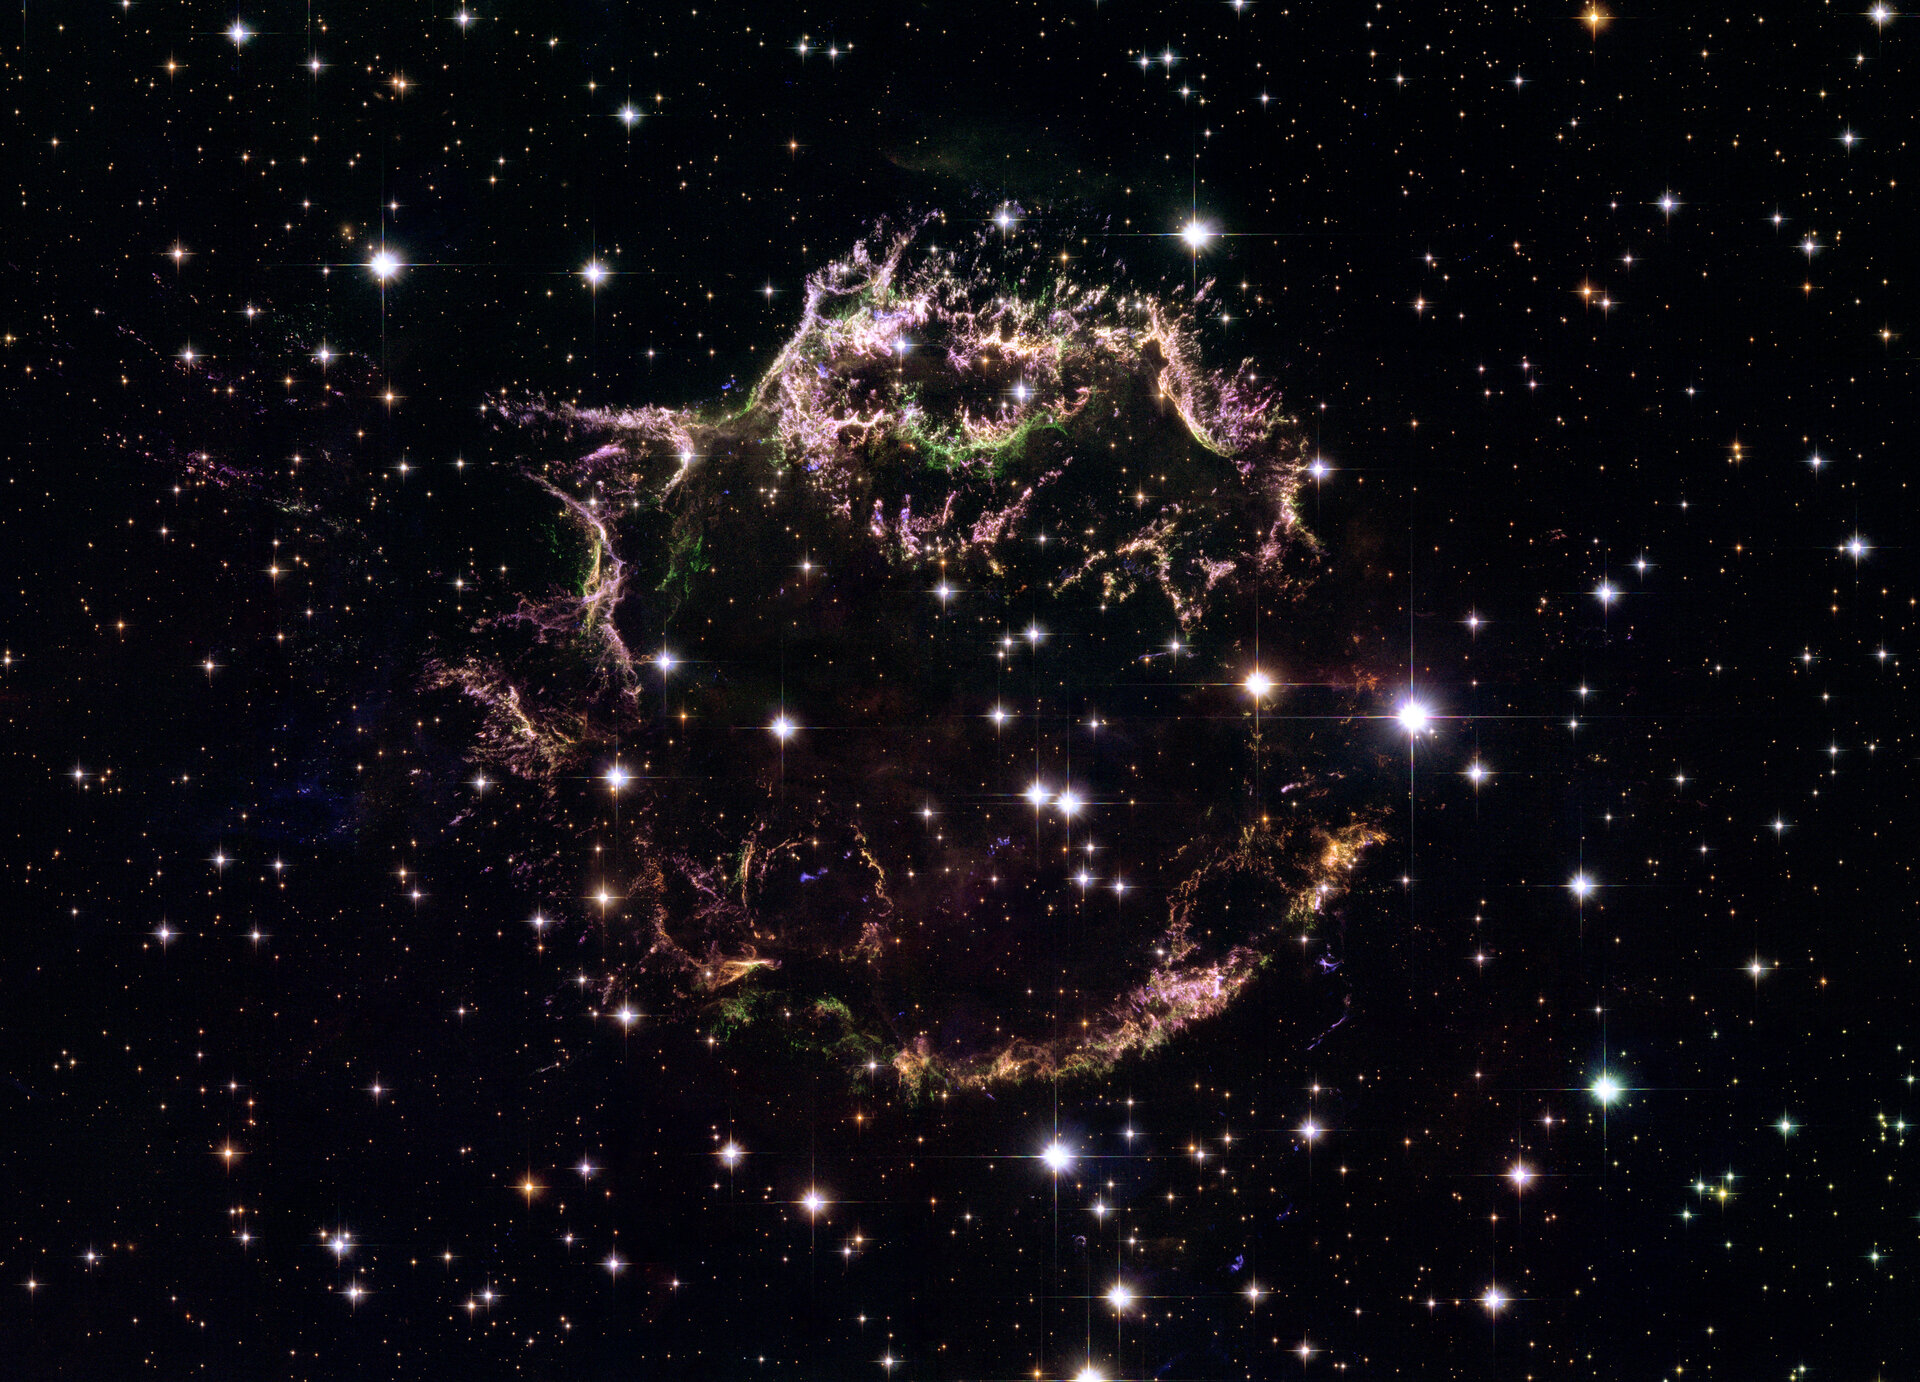
\includegraphics[width=0.7\linewidth]{figures/supernova1.jpg}
            \caption{Supernova}
            \label{fig:super}
        \end{figure}

    \end{columns}
\end{frame}

\begin{frame}{Antiteilchen}
    \begin{columns}[c]
        \column{.45\textwidth}
        \begin{itemize}
            \item Jedes Fermion hat ein Antiteilchen
                  \begin{exampleblock}{Dirac-Gleichung}
                      \[
                          \left( i \hbar \gamma^\mu \partial_\mu - m \right) \psi = 0
                      \]
                      Hierbei sind:
                      \begin{itemize}
                          \item \( \hbar \) das reduzierte Plancksche Wirkungsquantum,
                          \item \( \gamma^\mu \) die Gamma-Matrizen,
                          \item \( \partial_\mu \) der kovariante Ableitungsoperator,
                          \item \( m \) die Masse des Teilchens,
                          \item \( \psi \) der Dirac-Feldvektor.
                      \end{itemize}

                  \end{exampleblock}
        \end{itemize}
        \column{.4\textwidth}
        \begin{figure}
            \centering
            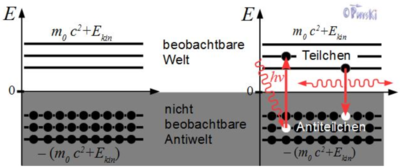
\includegraphics[width=1\linewidth]{figures/positron.png}
            \caption{Positron} \label{fig:positron}
        \end{figure}
    \end{columns}
\end{frame}
\subsection{Bosonen}
\begin{frame}{Feynman Diagramme}
    \begin{columns}
        \column{.45\textwidth}
        \begin{table}
            \centering
            \begin{tabular}{c|c}
                Fermion     & \feynmandiagram[horizontal=a to b]{a -- [fermion] b}; \\ \hline
                Antifermion & \feynmandiagram[horizontal=a to b]{b -- [fermion] a}; \\ \hline
                Photon      & \feynmandiagram[horizontal=a to b]{a -- [photon] b};  \\ \hline
                W-,Z-Boson  & \feynmandiagram[horizontal=a to b]{a -- [boson] b};   \\ \hline
                Gluon       & \feynmandiagram[horizontal=a to b]{a -- [gluon] b};   \\ \hline
                Skalarboson & \feynmandiagram[horizontal=a to b]{a -- [scalar] b};  % dazu gehört auch das Higgs Boson
            \end{tabular}
            \caption{Symbole im Feynmandiagramm}
            \label{tab:feynmandiagrams}
        \end{table}
        \pause
        \column{.45\textwidth}
        \begin{tikzpicture}
            \draw[->] (-0.5,-0.5) -- (-0.5, 3) node[right] {x};
            \draw[->] (-0.5,-0.5) -- (5,-0.5) node[above] {t};
            \feynmandiagram [horizontal=a to b] {
            f1 [particle=$e^{-}$] -- [fermion] a -- [fermion] f2 [particle=$e^{+}$],
            a -- [photon, edge label=$\gamma$] b,
            g1 [particle=$e^{+}$] -- [fermion] b -- [fermion] g2 [particle=$e^{-}$],
            };
        \end{tikzpicture}
    \end{columns}
\end{frame}

\begin{frame}{Bosonen Überblick}
    \begin{columns}[c]
        \column{.45\textwidth}
        \begin{block}{Spin von Bosonen}
            Bosonen haben immer einen ganzzahligen Spin ($0, 1, 2, ...$) % Pauli-Prinzip erwähnen (unterliegen diesem nicht)
        \end{block}
        \vspace{20pt}
        \textbf{Arten von Bosonen}
        \begin{itemize}
            \item Mesonen (Zusammengesetze Teilchen) % Hadronen erwähnen
            \item Elementarteilchen (siehe Abb.)
        \end{itemize}

        \column{.45\textwidth}
        \begin{figure}
            \centering
            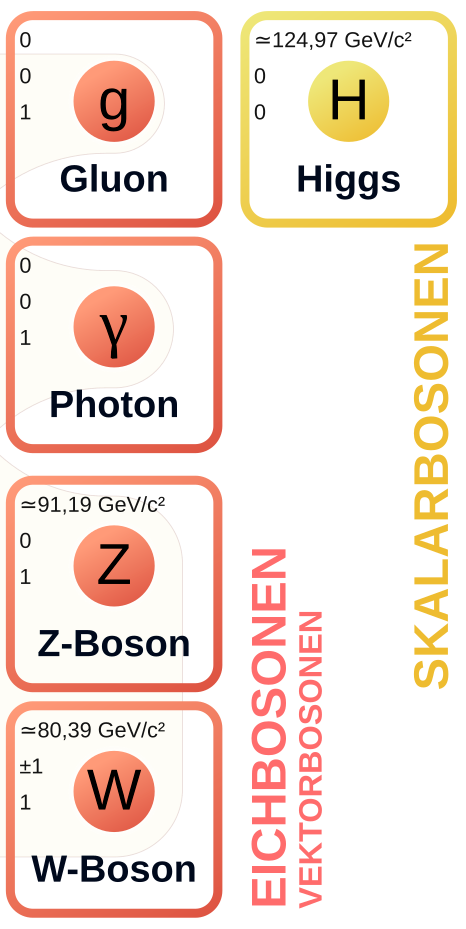
\includegraphics[width=0.45\linewidth]{figures/bosonen.png}
            \caption{Bosonen Überblick}
            \label{fig:bosonen}
        \end{figure}
    \end{columns}
\end{frame}

\begin{frame}{Mesonen}
    \begin{columns}[c]
        \column{.45\textwidth}
        \begin{itemize}
            \item Untergruppe der Hardonen
            \item instabile Teilchen
            \item Baryonenzahl $= 0$
        \end{itemize}
        \vspace{20pt}
        \begin{exampleblock}{Beispiele für Mesonen}
            \begin{itemize}
                \item Pion (siehe Abb.) % zuerst gefunden
                \item Tetraquarks
                \item Psion % dadurch wurde der Charm Quark endeckt
            \end{itemize}
        \end{exampleblock}
        \column{.45\textwidth}
        \begin{figure}
            \centering
            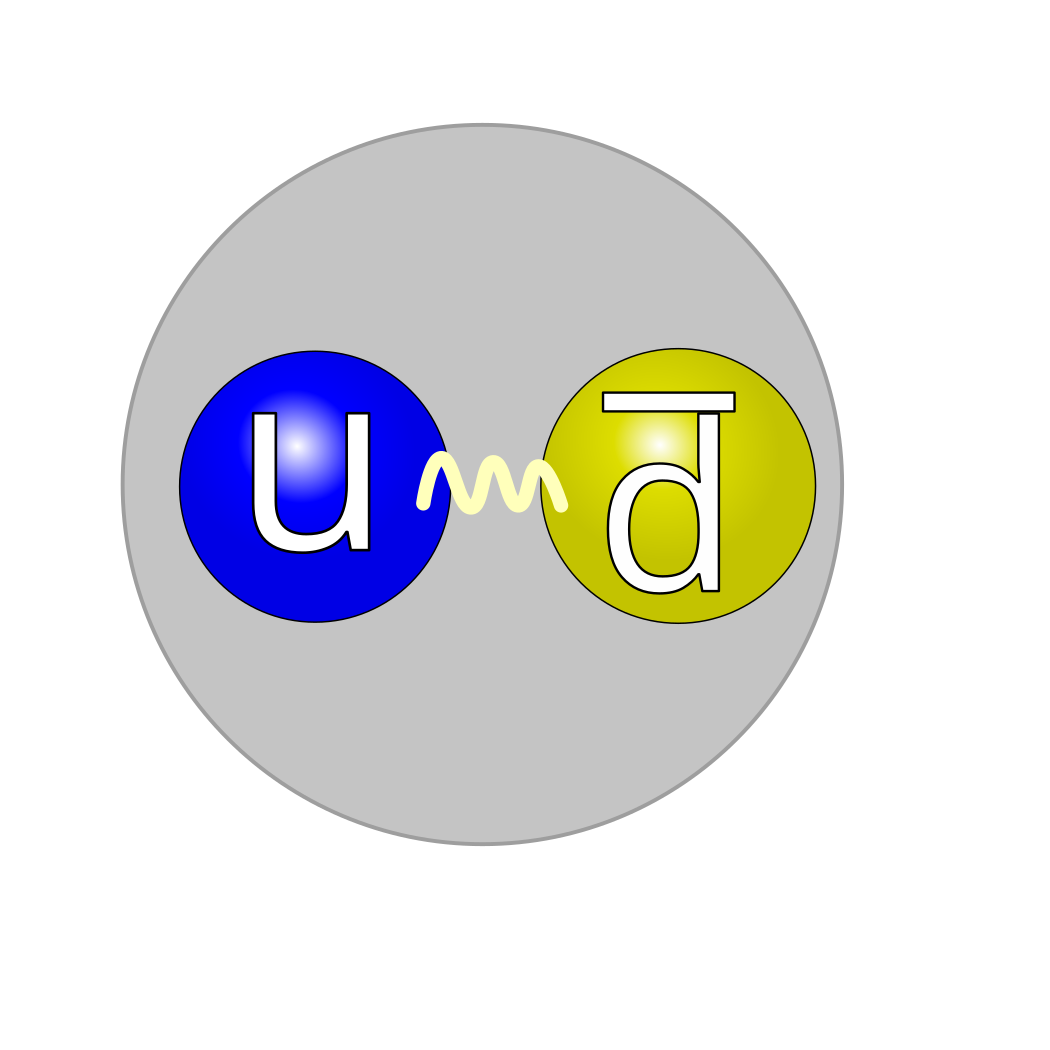
\includegraphics[width=0.4\linewidth]{figures/Pion.png}
            \feynmandiagram[small, horizontal=a to b]{
            a [particle=$\pi^0$] -- [scalar] b -- [fermion] c1 -- [fermion] c2 -- [fermion] b,
            c1 -- [photon] p1 [particle=$\gamma_1$],
            c2 -- [photon] p2 [particle=$\gamma_2$]
            };
            \caption{Pion}
            \label{fig:pion}
        \end{figure}
    \end{columns}
\end{frame}

\begin{frame}{Eichbosonen}
    \begin{alertblock}{Definition}
        \centering Vermittelung der fundamentalen Wechselwirkungen (außer Gravitation) \\
        Spin: $s=1$
    \end{alertblock}
    \vspace{10pt}
    \begin{table}
        \centering
        \begin{tabular}{c|c|c|c}
            \bf Boson          & Photon $\gamma$ & $W^\pm$-/$Z^0$-Boson & Gluon $g$  \\ \hline
            \bf Wechselwirkung & Elektromagn.    & Schwache             & Starke     \\ \hline
            \bf Eichgruppe     & $U(1)$          & $SU(2)$              & $SU(3)$    \\ \hline
            \bf Bosonenanzahl  & $1$             & $3$                  & $8$        \\ \hline
            \bf Ladung         & elek. Ladung    & schacher Isospin     & Farbladung
        \end{tabular}
        \caption{Eichbosonen}
        \label{tab:eichbosonen}
    \end{table}
\end{frame}

\begin{frame}{Eichgruppen}
    \begin{alertblock}{Symmetriegruppen}<2->
        $U(1)_Y \to$ Schwache Hyperladung | $SU(2)_L \to$ Flavour | $SU(3)_C \to$ Farbladung
    \end{alertblock}
    % exclude in handout!!!
    \begin{alertblock}{Symmetriegruppen}<only@1>
        \begin{itemize}
            \item $U(1)_Y \to$ Schwache Hyperladung
            \item $SU(2)_L \to$ Flavour
            \item $SU(3)_C \to$ Farbladung
        \end{itemize}
    \end{alertblock}
    \begin{columns}[c]
        \column{.45\textwidth}
        \begin{block}{Generatoren}<2->
            \begin{itemize}
                \item jede Gruppe besitzt Generatoren
                \item Anzahl der Generatoren = \\
                      Anzahl der Eichbosonen
            \end{itemize}
        \end{block}
        \vspace{10pt}
        \begin{block}{Starke Wechselwirkung}<3->
            $= SU(3)_C$ \\
            \begin{itemize}
                \item 8 Generatoren (Oktett)
            \end{itemize}
        \end{block}
        \column{.45\textwidth}
        \begin{block}{Elektroschwache Wechselwirkung}<4->
            $= SU(2)_L \times U(1)_Y$ \\
            \vspace{2pt}
            \textbf{Elektromagnetismus}
            \begin{itemize}
                \item $SU(2)_L \times U(1)_Y \to U(1)_{em}$
                \item $Q = T_3 + \frac{1}{2}Y_W$
                \item 1 Generator (Singlet)
            \end{itemize}
            \vspace{2pt}
            \textbf{Schwache Wechselwirkung}
            \begin{itemize}
                \item 3 Generatoren (Triplett)
            \end{itemize}
        \end{block}
    \end{columns}
\end{frame}

\begin{frame}{Photon}
    \begin{columns}[c]
        \column{.45\textwidth}
        \begin{block}{Korrespondierende Ladung}
            Elektromagnetische Ladung $Q = T_3 + \frac{1}{2}Y_W$ % Q bleibt immer erhalten, immer Vielfaches von e außer Quarks mit 1/3 e
        \end{block}
        \vspace{10pt}
        \begin{itemize}
            \item Ruhemasse: $m_0 = 0$ % unendlich Reichweite
            \item Geschwindigkeit: $c = 3 \cdot 10^8 \frac{m}{s}$
        \end{itemize}
        \vspace{10pt}
        \begin{exampleblock}{Entstehung}
            \begin{itemize}
                \item Synchrotonstrahlung
                \item Energieniveau-Übergang
                \item Annihilation
            \end{itemize}
        \end{exampleblock}
        \pause
        \column{.45\textwidth}
        \textbf{Teilchen der elektromagn. Strahlung}
        \vspace{10pt}
        \begin{figure}
            \centering
            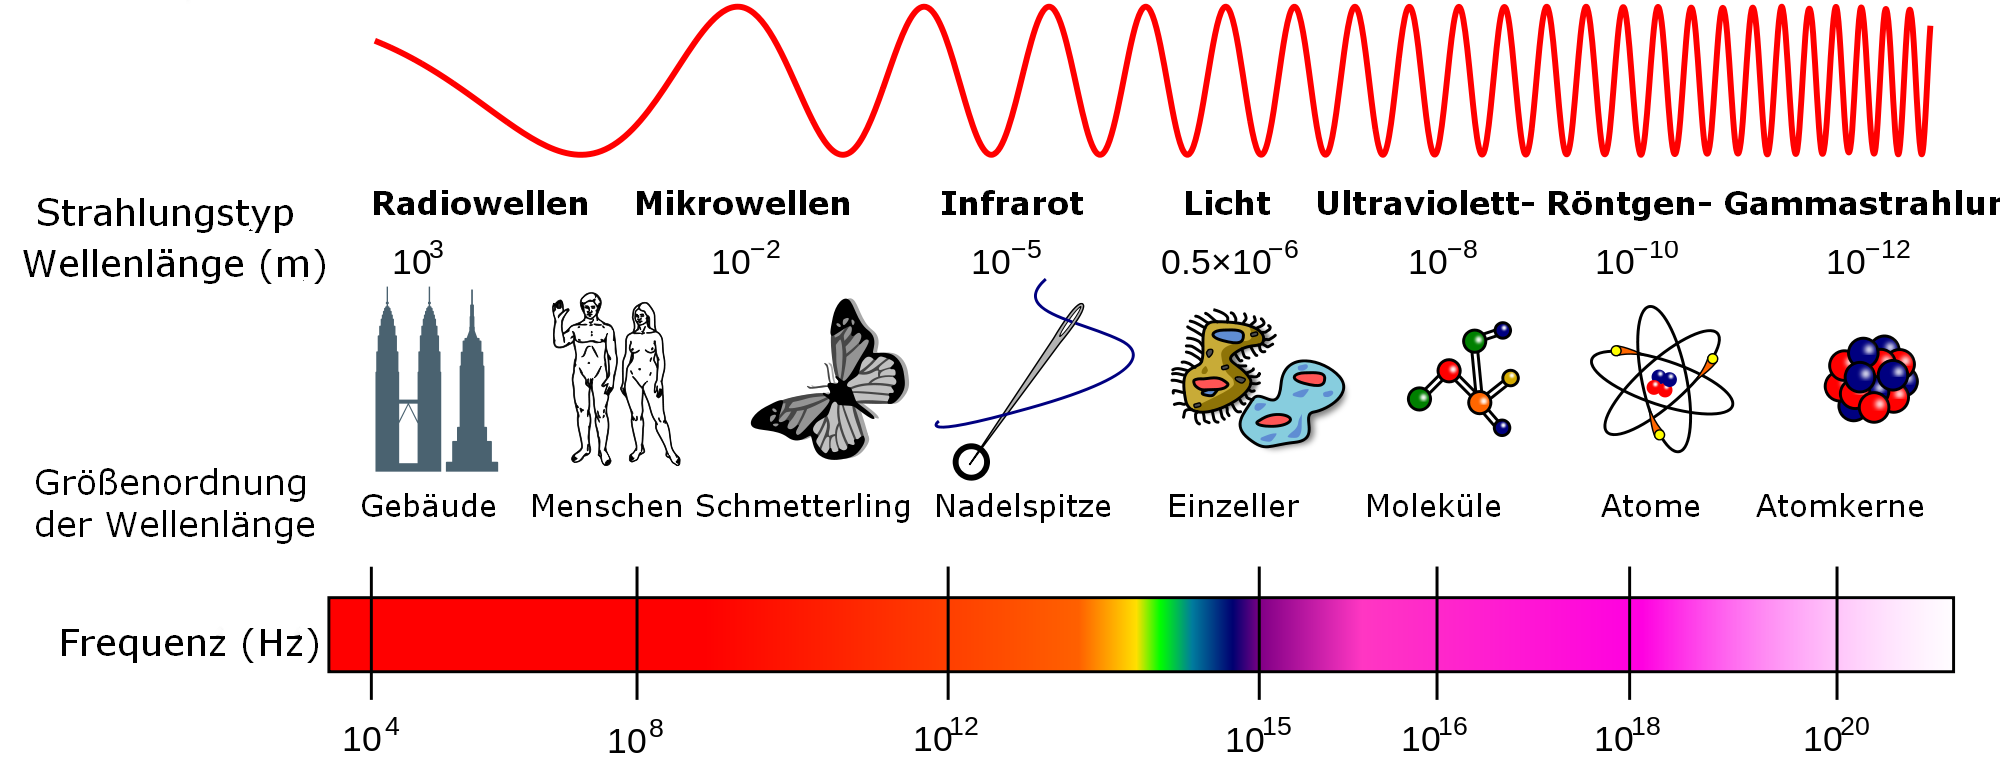
\includegraphics[width=1\linewidth]{figures/elekmagnstrahlung.png}
            \caption{Elektromagnetische Strahlung}
            \label{fig:elekmagnstrahlung}
        \end{figure}
    \end{columns}
\end{frame}

\begin{frame}{Photon: Feynman-Diagramme}
    \begin{columns}[c]
        \column{.45\textwidth}
        \begin{figure}
            \centering
            \feynmandiagram[vertical=a to b]{
            e1 [particle=$e^-$] -- [fermion] a,
            e2 [particle=$e^-$] -- [fermion] b,
            a -- [photon, edge label=$\gamma$] b,
            a -- [fermion] e3 [particle=$e^-$],
            b -- [fermion] e4 [particle=$e^-$]
            };
            \caption{Abstoßung von 2 Elektronen}
            \label{fig:abstossung}
        \end{figure}
        \pause
        \column{.45\textwidth}
        \begin{figure}
            \centering
            \feynmandiagram [horizontal=a to b] {
            e1 [particle=$e^{-}$] -- [fermion] a -- [fermion] e2 [particle=$e^{+}$],
            a -- [photon, edge label=$\gamma$] b,
            e3 [particle=$\mu^{+}$] -- [fermion] b -- [fermion] e4 [particle=$\mu^{-}$],
            };
            \caption{\centering Annihilation von einem Elektron und Positron}
            \label{fig:annihilation}
        \end{figure}
    \end{columns}
\end{frame}

\begin{frame}{W- und Z-Bosonen}
    \begin{columns}[c]
        \column{.45\textwidth}
        \begin{block}{Korrespondierende Ladung}
            Schwacher Isospin $T_3$
        \end{block}
        \vspace{10pt}
        \begin{itemize}
            \item Teilchen: $W^+$, $W^-$, $Z^0$
            \item $W^\pm$ übertragen elek. Ladung % Z^0 ist neutral
                  %w+ und W- sind gegenseitig ihr Antiteilchen, Z0 ist sein eigenes Antiteilchen
            \item hohe Masse: $m_0 > 80 \frac{GeV}{c^2}$ % fast 80 Mal so schwer wie ein proton = Fe
                  \\ $\implies$ geringe Reichweite
        \end{itemize}
        \vspace{10pt}
        \begin{exampleblock}{Vorkommen}
            \begin{itemize}
                \item $W^\pm$: Beta+/- Zerfall
                \item $Z^0$: elastische Neutrino Streuung
            \end{itemize}
        \end{exampleblock}
        \pause
        \column{.5\textwidth}
        \begin{table}
            \centering
            \small
            \begin{tabular}{c|c|c}
                             & \bf Rechtshändig                 & \bf Linkshändig               \\ \hline
                Helizität    & positiv                          & negativ                       \\ \hline
                Spinrichtung & in $\overrightarrow{p}$ Richtung & entgegen $\overrightarrow{p}$ \\ \hline
                Interaktion  & Antiteilchen                     & Teilchen
            \end{tabular}
            \label{tab:helizitaet}
        \end{table}
        \begin{figure}
            \centering
            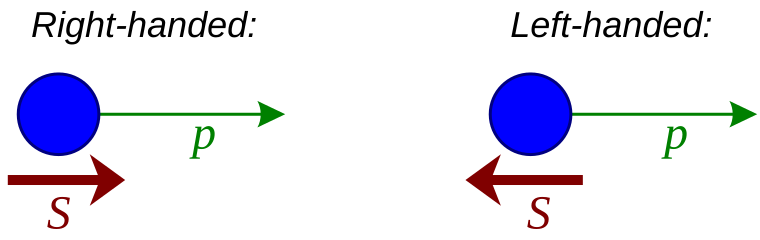
\includegraphics[width=0.95\linewidth]{figures/lefthanded.png}
            \caption{Helizität eines Teilchen}
            \label{fig:helizitaet}
        \end{figure}
    \end{columns}
    %Relation mit $T_3$: $Q = T_3 + \frac{1}{2} Y_W$
\end{frame}

\begin{frame}{W- und Z-Bosonen: Feynman-Diagramme}
    \begin{columns}[c]
        \column{.45\textwidth}
        \begin{figure}
            \centering
            \feynmandiagram[horizontal=d to a, tree layout]{
            d [particle=$d$] -- [fermion] a,
            a -- [boson, edge label=$W^-$] w1,
            a -- [fermion] u1 [particle=$u$],
            v1 [particle=$\overline{\nu}_e$] -- [fermion] w1,
            w1 -- [fermion] e1 [particle=$e^-$]
            };
            \caption{Beta-Minus-Zerfall}
            \label{fig:betazerfall}
        \end{figure}
        \pause
        \column{.45\textwidth}
        \begin{figure}
            \centering
            \feynmandiagram[vertical=a to b]{
            e1 [particle=$e^-$] -- [fermion] a,
            v1 [particle=$\nu_e$] -- [fermion] b,
            a -- [boson, edge label=$Z^0$] b,
            b -- [fermion] v2 [particle=$\nu_e$],
            a -- [fermion] e2 [particle=$e^-$]
            }; % Neutrinos können nur E, p und s austauschen
            \caption{\centering Neutrino-Elektron-Interaktion via $Z^0$ Boson}
            \label{fig:z0}
        \end{figure}
    \end{columns}
\end{frame}

\begin{frame}{Gluon}
    \begin{columns}[c]
        \column{.45\textwidth}
        \begin{block}{Korrespondierende Ladung}
            Farbladung $C$
        \end{block}
        \vspace{10pt}
        % color cycle => SU(3)
        % different colors attract each other
        % there are positive and negative colors
        % quarks have positive and antiquarks negative
        \begin{itemize}
            \item als masselos angenommen
            \item es gibt 8 Gluonen mit verschiedenen Farbzuständen
            \item Gluonen besitzen immer eine Farbe und Antifarbe
            \item sie übertragen Farbladung
            \item Experimenteller Nachweis (1979): PETRA am Desy (3-Jet-Struktur)
        \end{itemize}
        %\textbf{Warum wirkt die starke WW nicht bei langen Distanzen?}
        \column{.45\textwidth}
        \begin{figure}
            \centering
            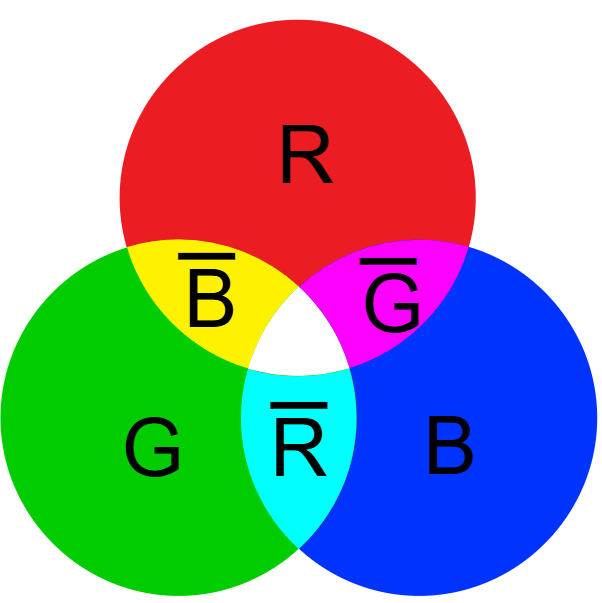
\includegraphics[width=0.35\linewidth]{figures/colors.png}
            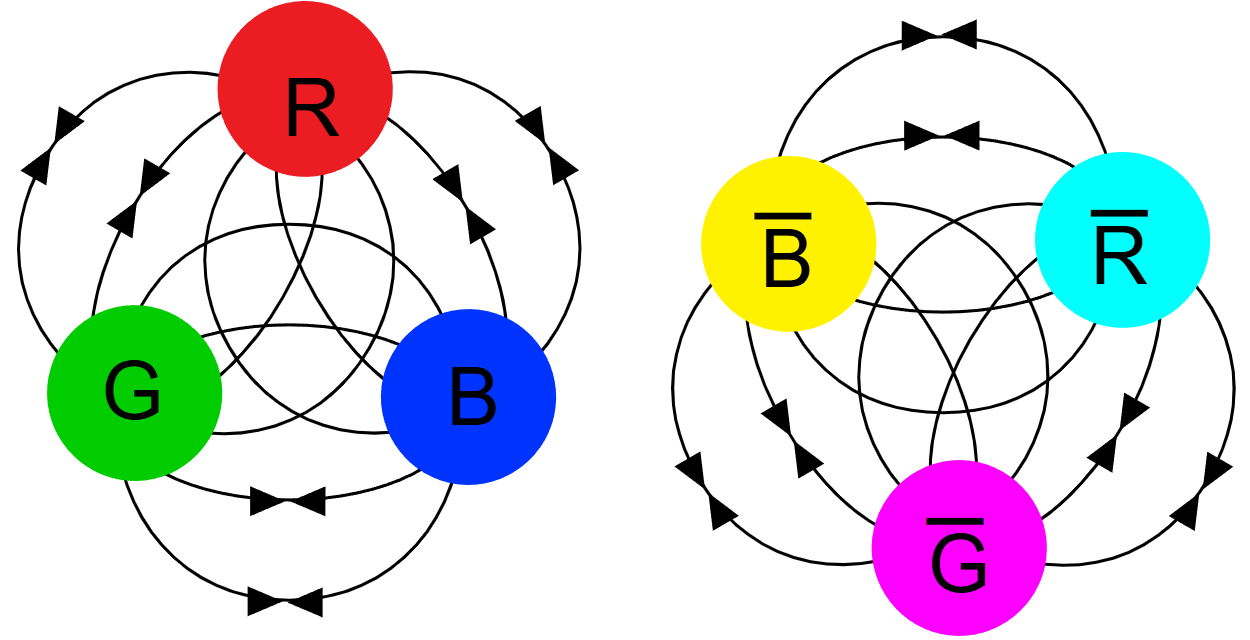
\includegraphics[width=0.8\linewidth]{figures/colorcharge.png}
            \caption{Farbladung}
            \label{fig:colorcharge}
        \end{figure}
    \end{columns}
\end{frame}

\begin{frame}{Gluon: Feynman-Diagramme}
    \begin{columns}[c]
        \column{.45\textwidth}
        \begin{figure}
            \centering
            \feynmandiagram[horizontal=d to a, layered layout]{
            d [blue, particle=$u$] -- [blue, fermion] a,
            a -- [boson, edge label=$g: b\overline{r} \ (\text{\color{blue} blau, \color{cyan} antirot})$] w1,
            a -- [red, fermion] u1 [red, particle=$u$],
            v1 [red, particle=$d$] -- [red, fermion] w1,
            w1 -- [blue, fermion] e1 [blue, particle=$d$]
            };
            \caption{Gluon Austausch}
            \label{fig:gluon1}
        \end{figure}
        \column{.45\textwidth}
        \pause
        \begin{figure}
            \centering
            \feynmandiagram[vertical=a to b]{
            e1 [blue, particle=$u$] -- [blue, fermion] a,
            v1 [red, particle=$d$] -- [red, fermion] b,
            a -- [boson, edge label=$g: r\overline{b} + b\overline{r}$] b,
            b -- [blue, fermion] v2 [blue, particle=$d$],
            a -- [red, fermion] e2 [red, particle=$u$]
            }; % Neutrinos können nur E, p und s austauschen
            \caption{Gluon Austausch}
            \label{fig:gluon2}
        \end{figure}
    \end{columns}
\end{frame}

\begin{frame}{Higgs-Boson}
    \begin{columns}[c]
        \column{.45\textwidth}
        \begin{block}{Funktion}
            Elementarteilchen erhalten ihre Masse durch Interaktion mit dem Higgs-Feld
        \end{block}
        \vspace{10pt}
        \textbf{Eigenschaften}
        \begin{itemize}
            \item Spin: $s=0 \implies$ Skalarboson
            \item hohe Masse: $m_0 = 124.97 \frac{GeV}{c^2}$
        \end{itemize}
        \vspace{10pt}
        $\implies$ spontane Symmetrie Brechung bei der elektro-schwachen WW wodurch $W^\pm, Z^0$ Masse erhalten
        \column{.45\textwidth}
        \pause
        \begin{exampleblock}{Entdeckung}
            \begin{itemize}
                \item \textbf{1964}: Theorie: Higgs-Mechanismus
                \item \textbf{1984}: Bau des LHC am CERN
                \item \textbf{2008}: Inbetriebnahme des LHC
                \item \textbf{2010}: Datensammlung durch ATLAS und CMS startet
                \item \textbf{2011}: Hinweise auf Higgs-Boson bei $125 \frac{GeV}{c^2}$ gefunden
                \item \textbf{2012}: Higgs-Entdeckung mit $5 \sigma$ bestätigt
                \item \textbf{2013}: Nobelpreis: Higgs, Englert
            \end{itemize}
        \end{exampleblock}
    \end{columns}
\end{frame}

\begin{frame}{Higgs-Boson: Feynman-Diagramme}
    \begin{columns}[c]
        \column{.45\textwidth}
        \begin{figure}
            \centering
            \feynmandiagram[horizontal=a to b]{
            a -- [fermion, edge label=$\overline{t}$] t1,
            t2 -- [fermion, edge label=$t$] a,
            t1 -- [fermion, edge label=$t$] t3,
            t4 -- [fermion, edge label=$\overline{t}$] t2,
            g1 [particle=$g$] -- [gluon] t1,
            g2 [particle=$g$] -- [gluon] t2,
            a -- [scalar, edge label=$H^0$] b
            };
            \caption{Erzeugung eines Higgs-Bosons durch 2 Gluonen}
            \label{fig:higgserzeugung}
        \end{figure}
        \column{.45\textwidth}
        \pause
        \begin{figure}
            \centering
            \feynmandiagram[small, horizontal=a to b, tree layout]{
            a -- [scalar, edge label=$H^0$] b,
            b -- [boson, edge label=$Z^0$] z1,
            b -- [boson, edge label=$Z^0$] z2,
            z1 -- [fermion] l1 [particle=$L^-$],
            l2 [particle=$L^+$] -- [fermion] z1,
            z2 -- [fermion] l3 [particle=$L^-$],
            l4 [particle=$L^+$] -- [fermion] z2
            };
            \caption{Zerfall eines Higgs-Bosons in 4 Leptonen}
            \label{fig:higgszerfall}
        \end{figure}
    \end{columns}
\end{frame}

\begin{frame}{Standardmodell}
    \begin{figure}
        \centering
        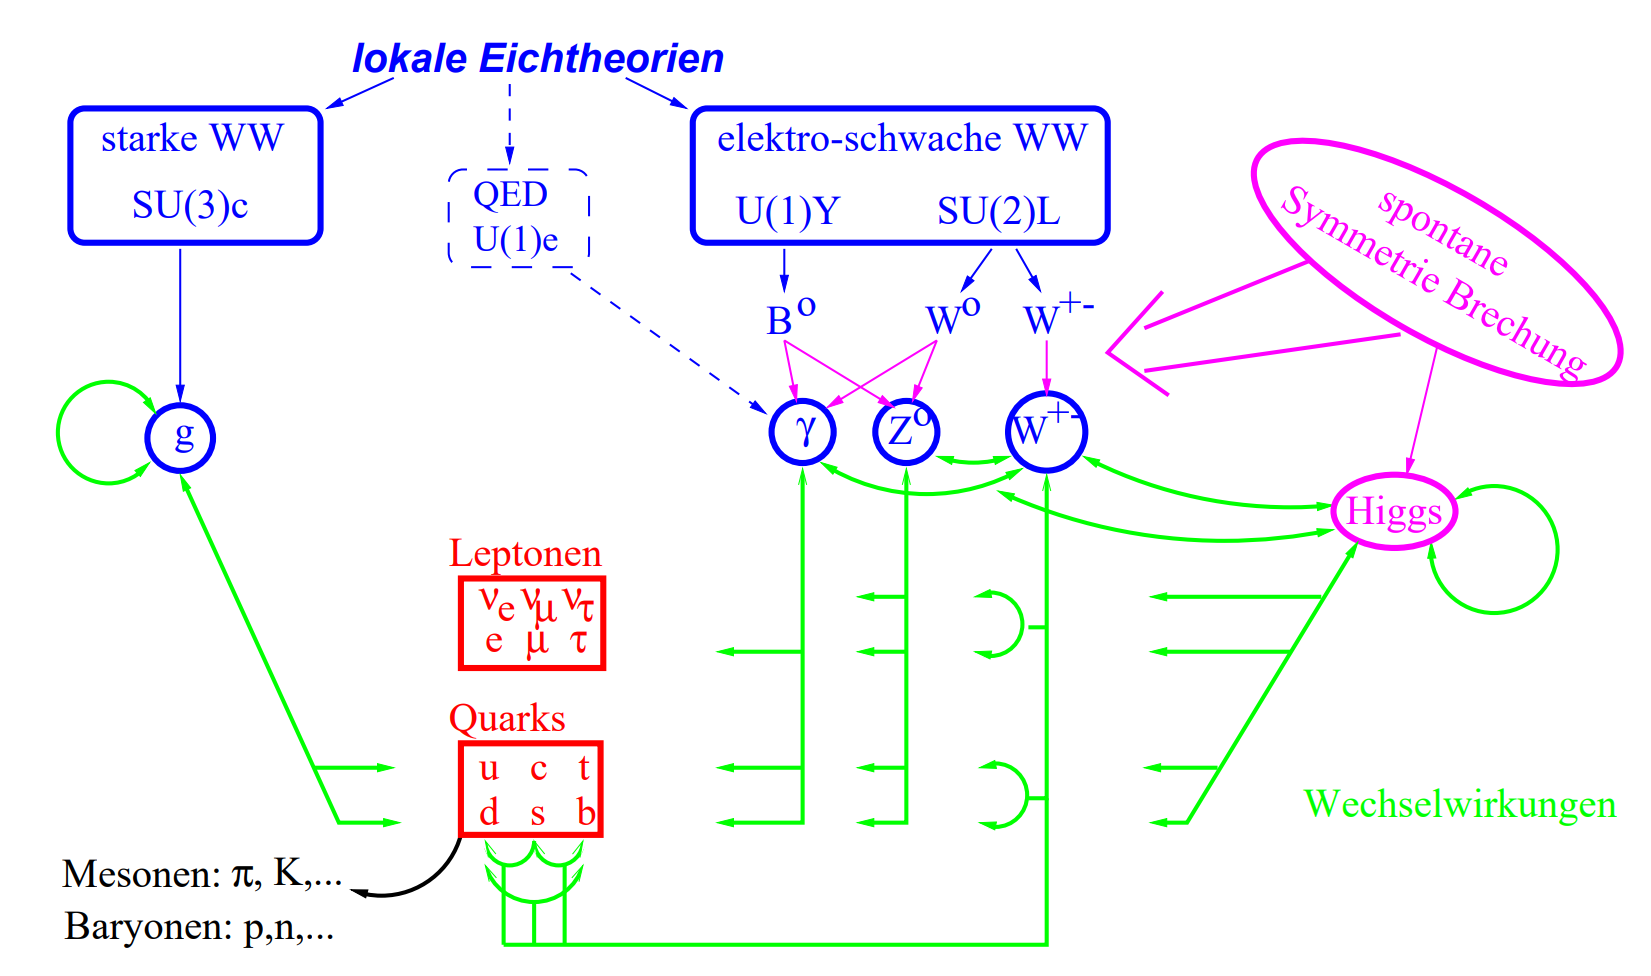
\includegraphics[width=0.7\linewidth]{figures/standardmodell.png}
        \caption{Standardmodell}
        \label{fig:sm}
    \end{figure}
\end{frame}

\begin{frame}{Fundamentale Wechselwirkungen}
    \begin{table}
        \centering
        \begin{tabular}{c|c|c|c}
            \bf Wechselwirkung       & \bf Reichweite   & \bf relative Stärke & \bf Austauschteilchen   \\ \hline
            Starke (QCD)             & $\sim 10^{-15}m$ & $1$                 & Gluonen                 \\ \hline
            Elektromagnetische (QED) & $\infty$         & $10^{-2}$           & Photonen                \\ \hline
            Schwache                 & $\sim 10^{-18}m$ & $10^{-15}$          & W- und Z-Bosonen        \\ \hline
            Gravitative              & $\infty$         & $10^{-41}$          & Graviton (hypothetisch)
        \end{tabular}
        \caption{Fundamentale Wechselwirkungen}
        \label{tab:wechselwirkungen}
    \end{table}
\end{frame}

\newcommand{\checkE}{\emoji{check-mark-button}}
\newcommand{\crossE}{\emoji{cross-mark}}
\begin{frame}{Fundamentale Wechselwirkungen}
    \begin{table}
        \centering
        \begin{tabular}{c|c|c|c}
            \bf Wechselwirkung       & \bf Quarks & \bf Leptonen ohne Neutrinos & \bf Neutrinos \\ \hline
            Starke (QCD)             & \checkE    & \crossE                     & \crossE       \\ \hline
            Elektromagnetische (QED) & \checkE    & \checkE                     & \crossE       \\ \hline
            Schwache                 & \checkE    & \checkE                     & \checkE       \\ \hline
            Gravitative              & \checkE    & \checkE                     & \checkE
        \end{tabular}
        \caption{Fundamentale Wechselwirkungen}
        \label{tab:wechselwirkungen2}
    \end{table}
\end{frame}

\begin{frame}{Theory of Everything?}
    \begin{figure}
        \centering
        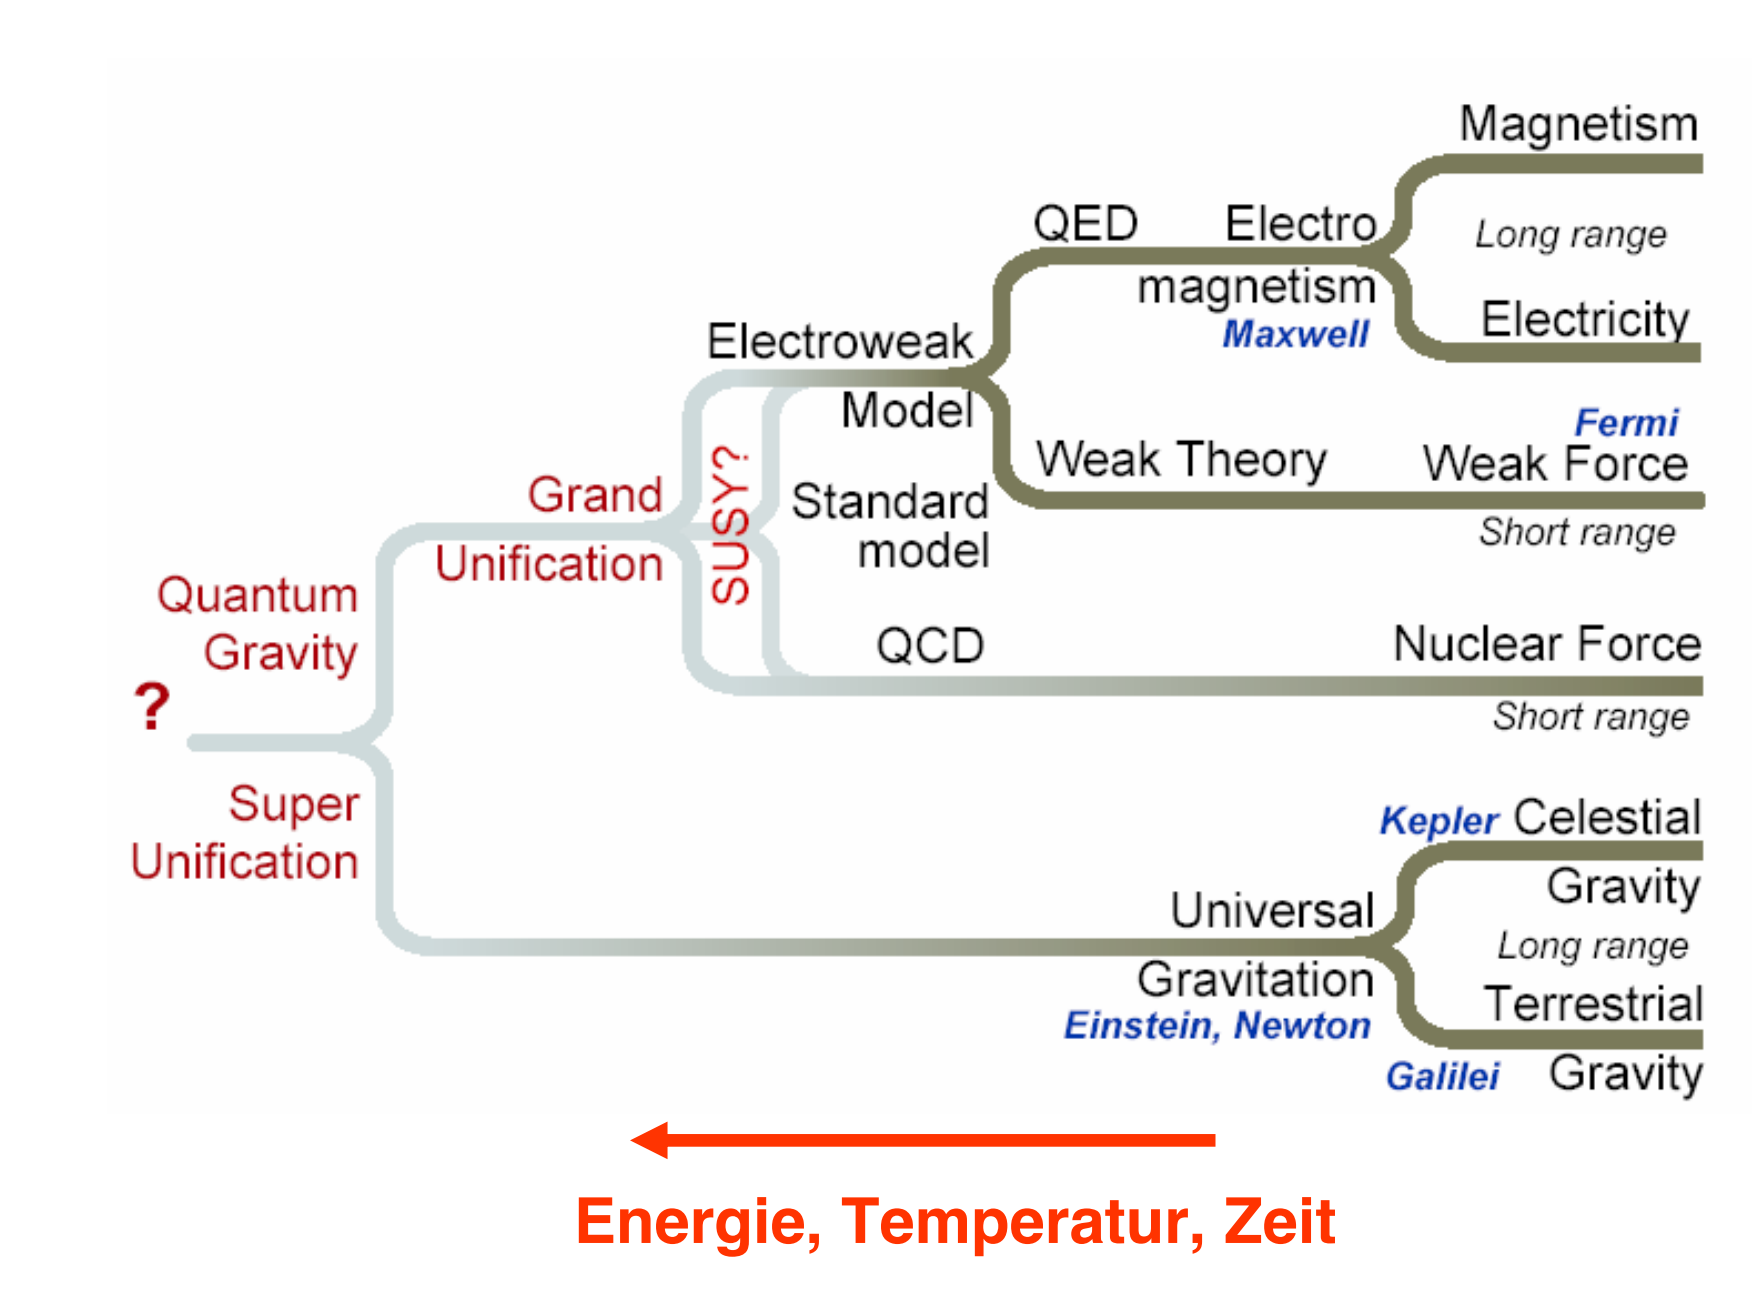
\includegraphics[width=0.65\linewidth]{figures/toe.png}
        %\caption{Theory of Everything}
        \label{fig:toe}
    \end{figure}
\end{frame}

\section{Teilchenbeschleuniger}
\begin{frame}{Streuexperimente}
    \begin{columns}[c]
        \column{.5\textwidth}
        \begin{figure}
            \centering
            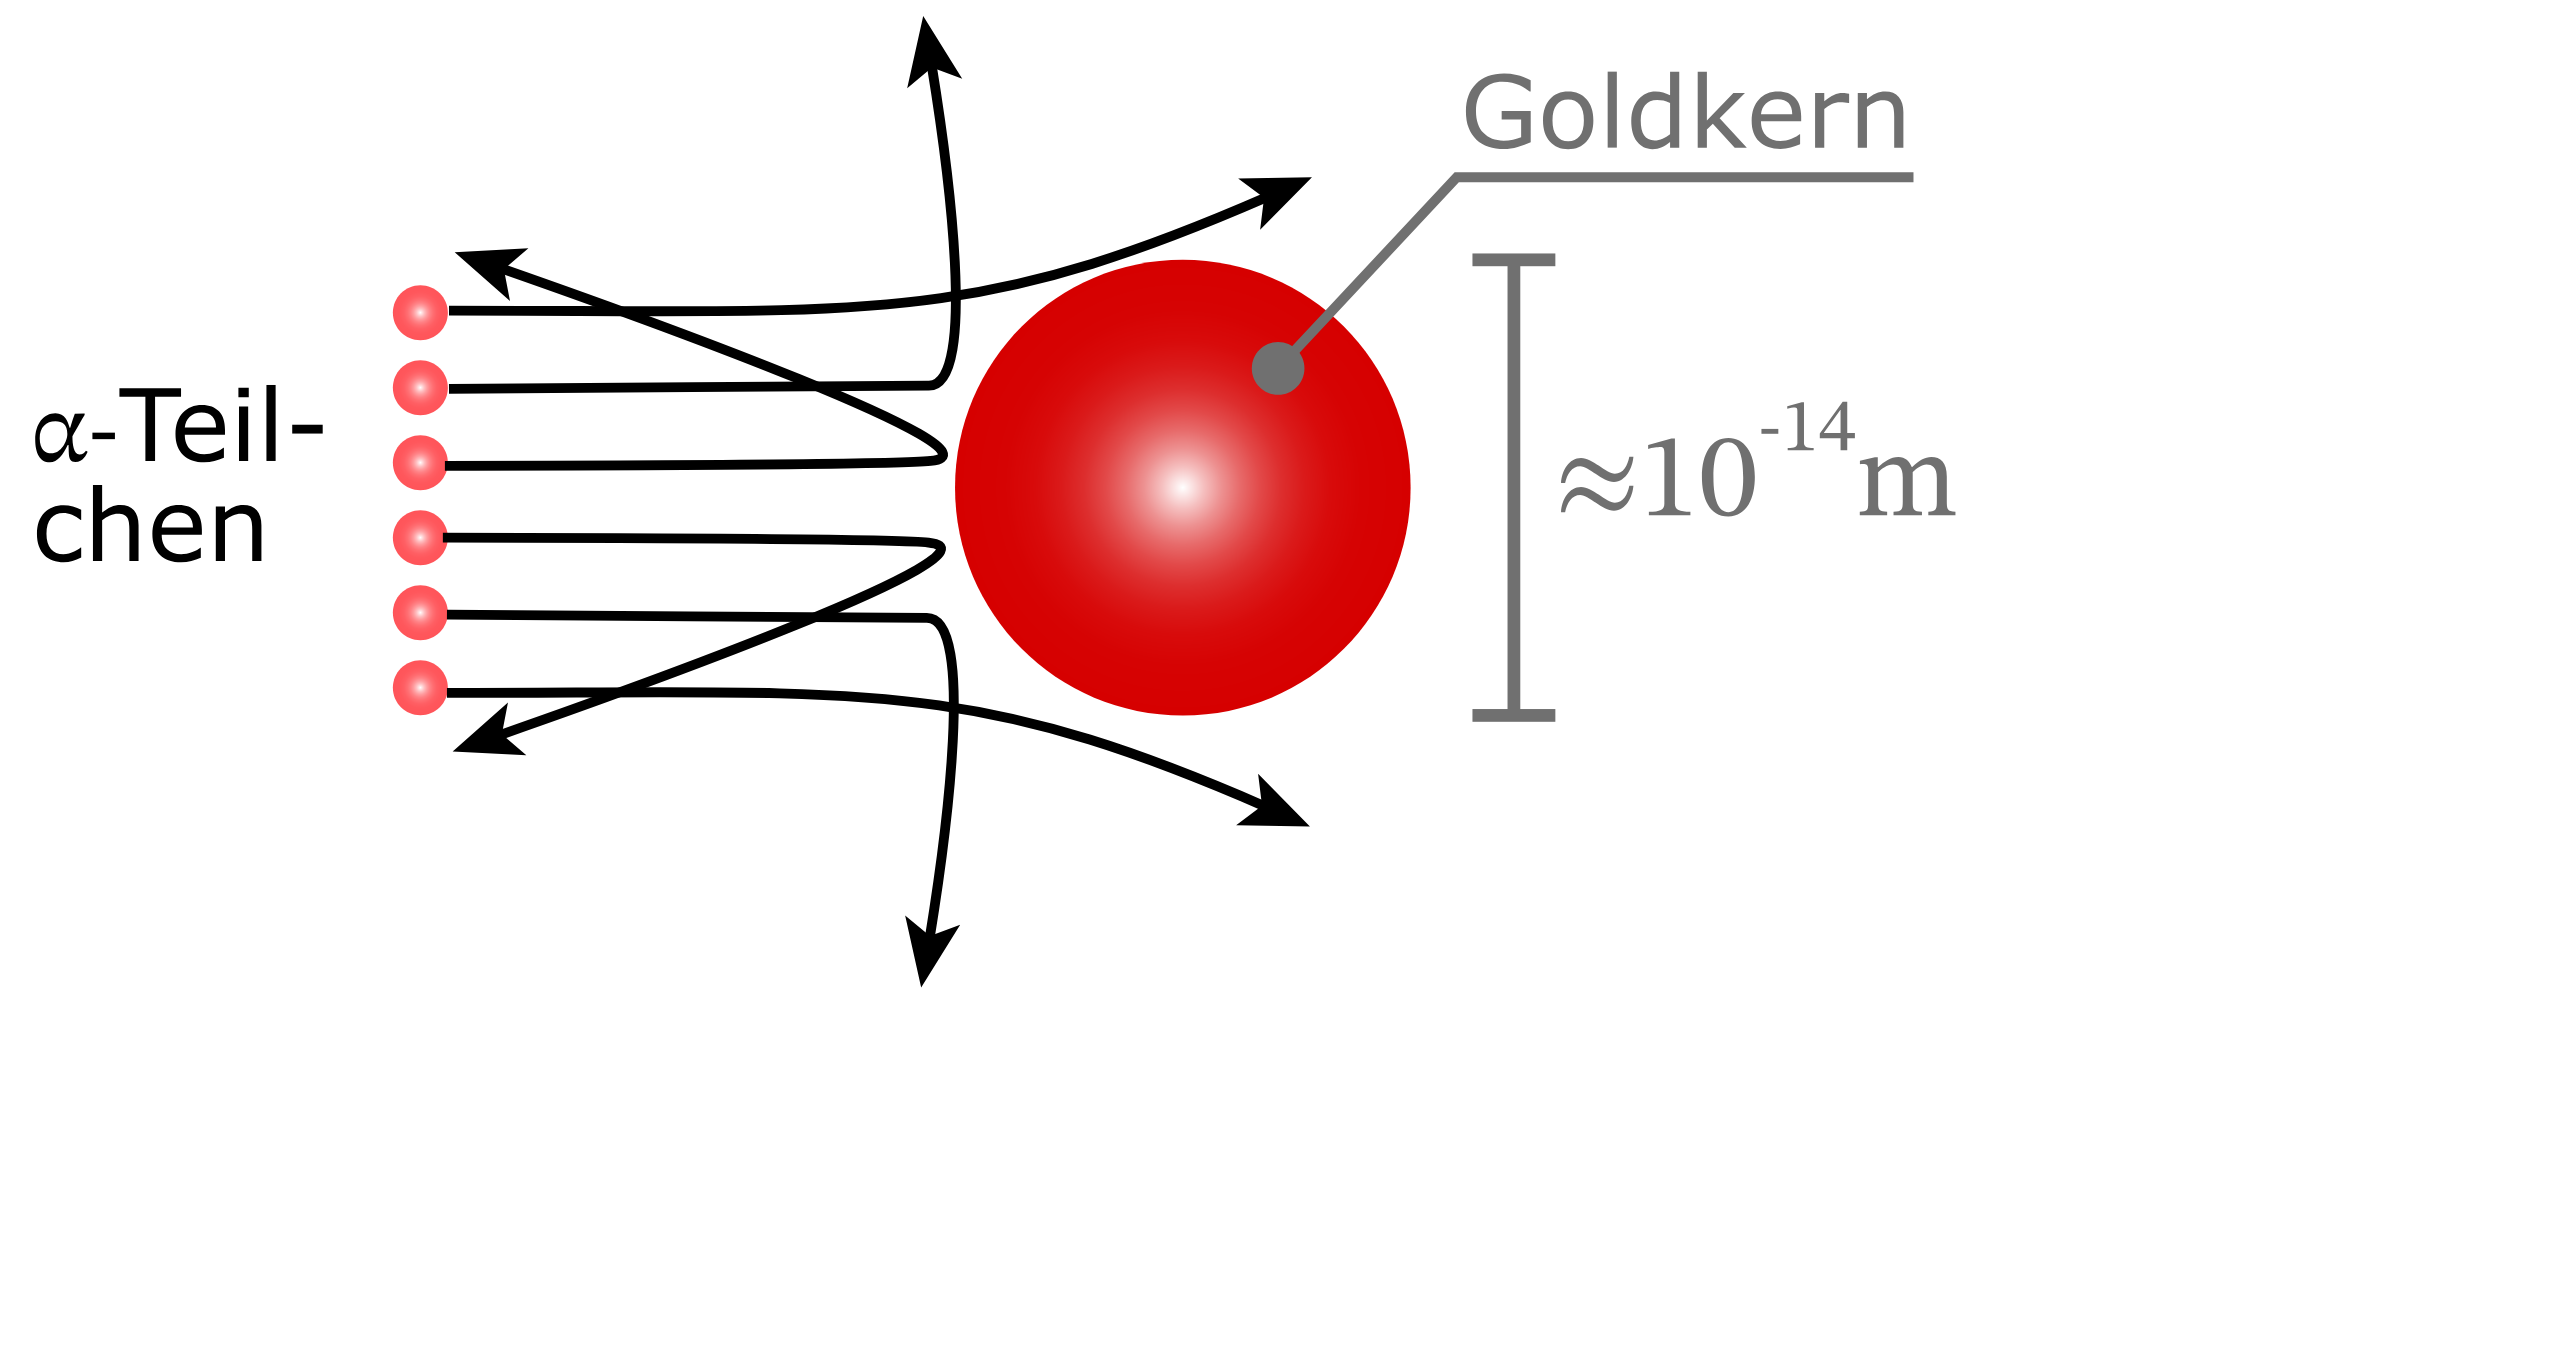
\includegraphics[width=1\linewidth]{figures/streuprozess2.png}
            \caption{Streuung am Goldkern}
            \label{fig:Streuung am Goldkern}
        \end{figure}

        \column{.5\textwidth}
        \begin{figure}
            \centering
            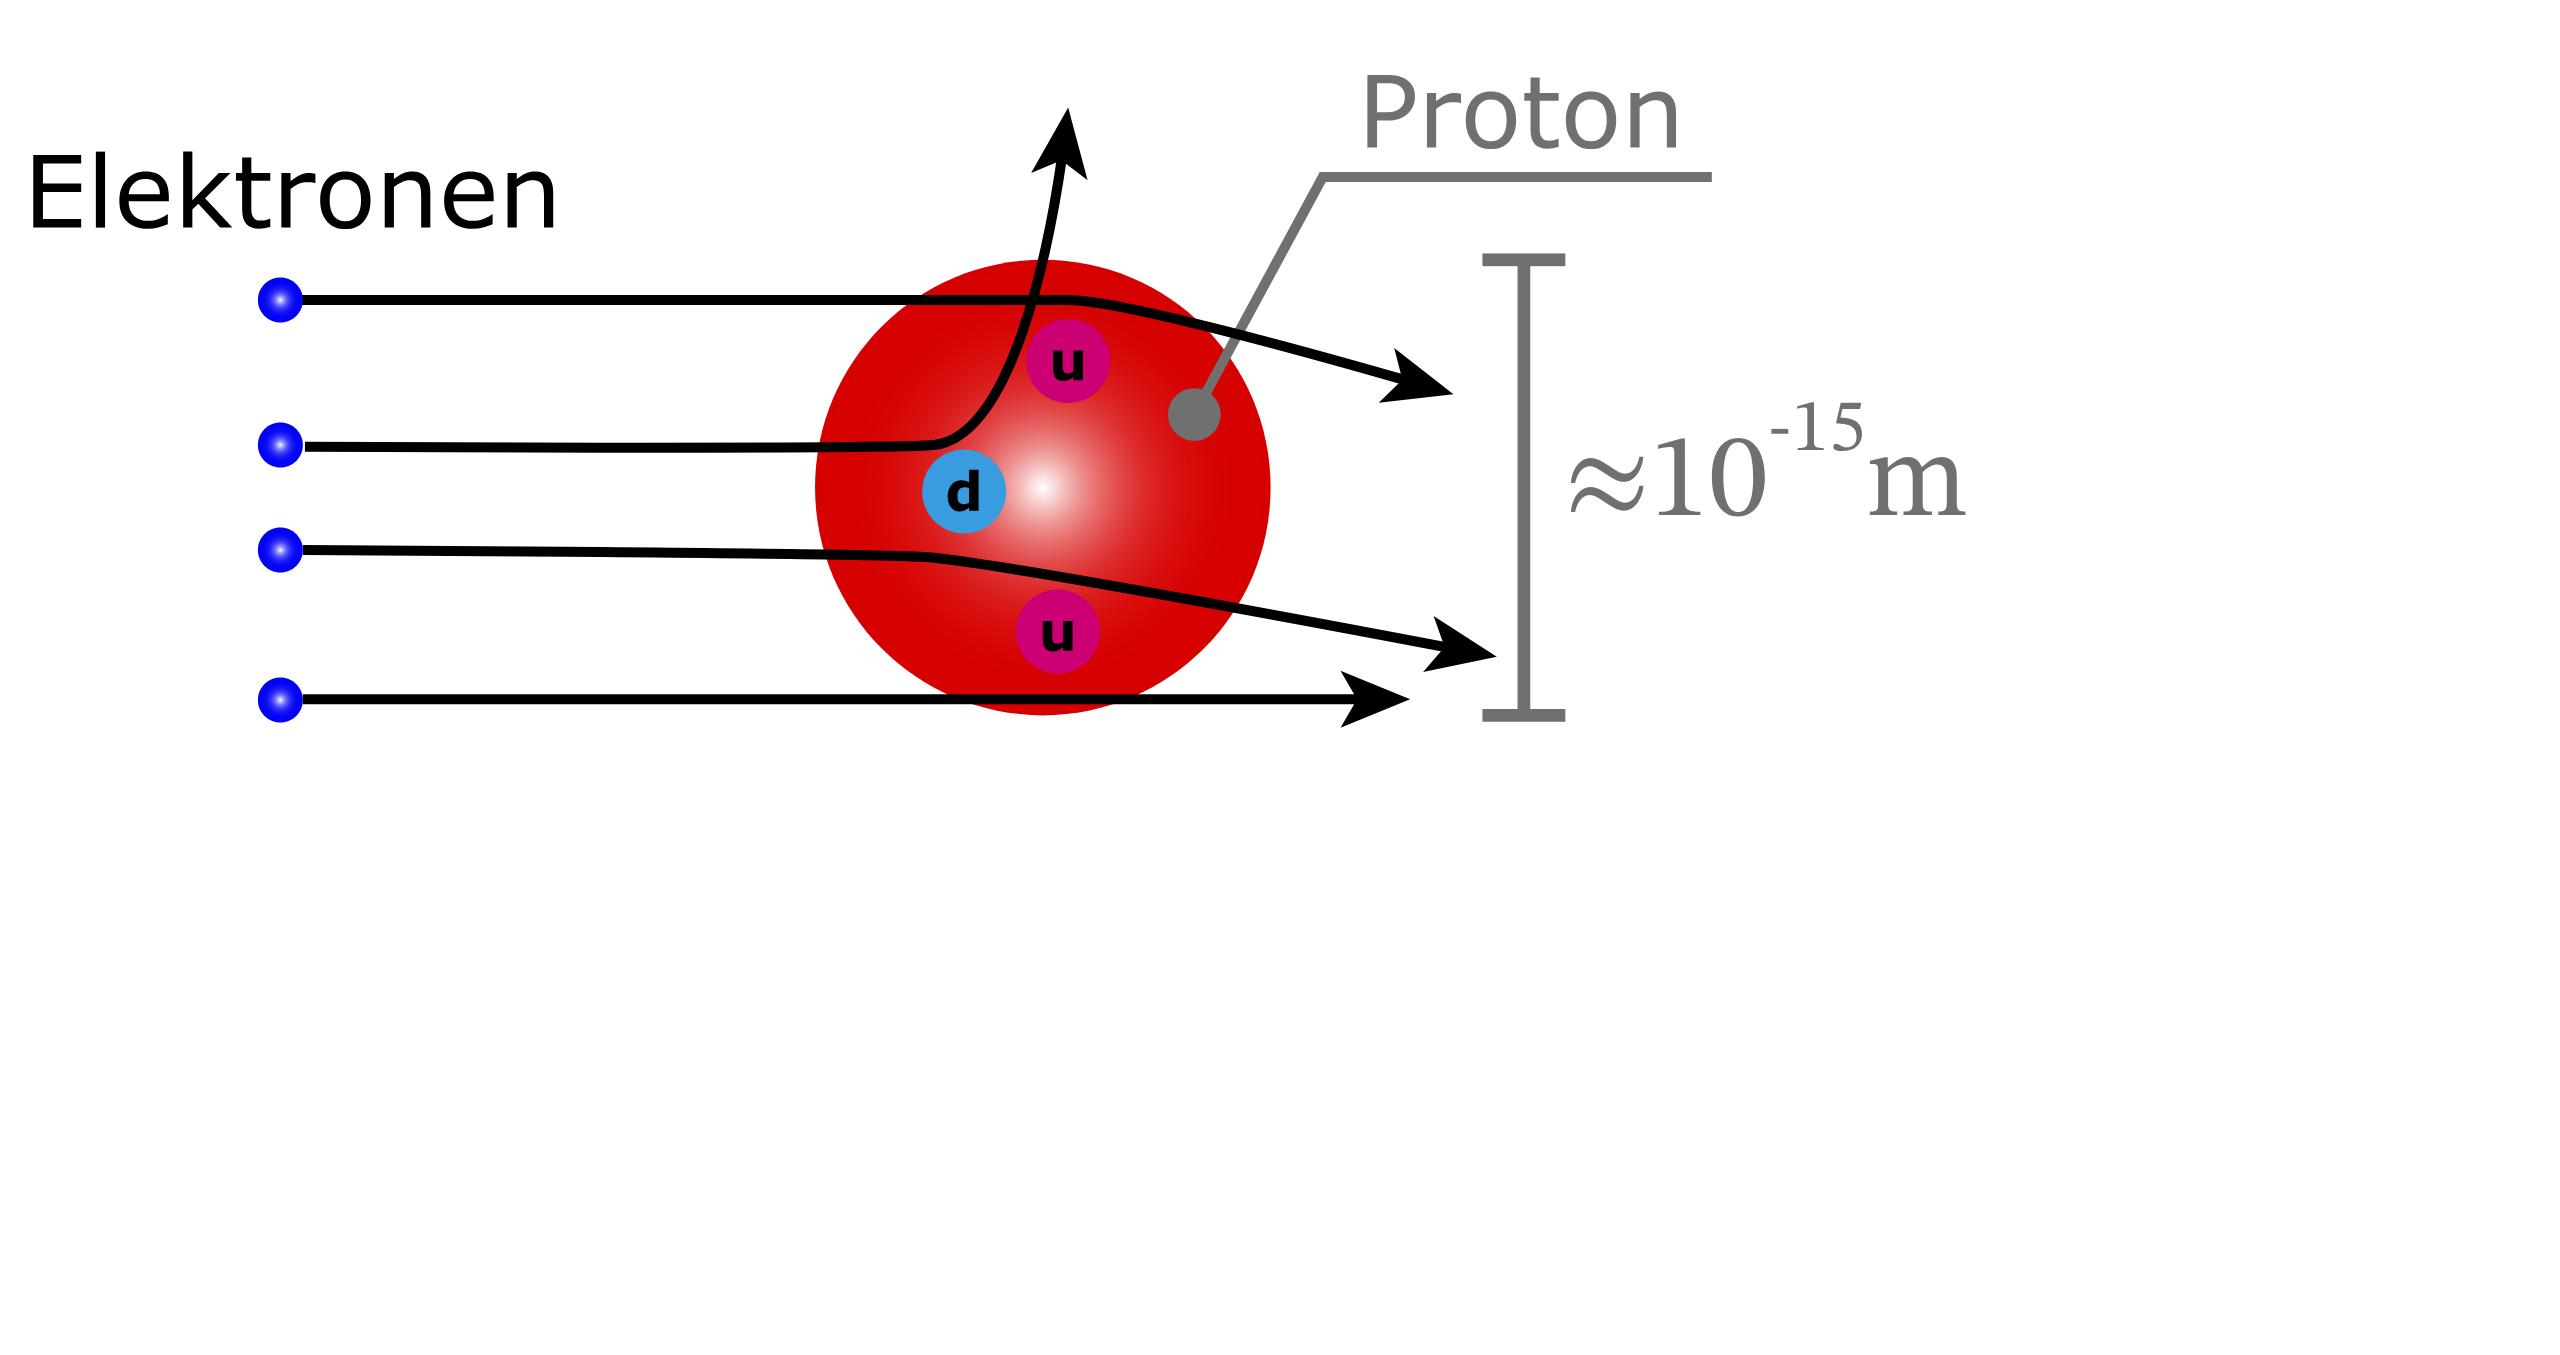
\includegraphics[width=1\linewidth]{figures/streuprozess1.png}
            \caption{Steuung an Quarks}
            \label{fig:Steuung an Quarks}
        \end{figure}

    \end{columns}
\end{frame}
\begin{frame}{Teilchenbeschleuniger}
    \begin{columns}[c]
        \column{.45\textwidth}
        \begin{itemize}
            \item annähernd Lichtgeschwindigkeit
            \item Spurendetektor Ionisation am Halbleiter
            \item Kalorimeter
            \item Identifikation
            \item Rekonstruktion

        \end{itemize}

        \column{.45\textwidth}
        \begin{figure}
            \centering
            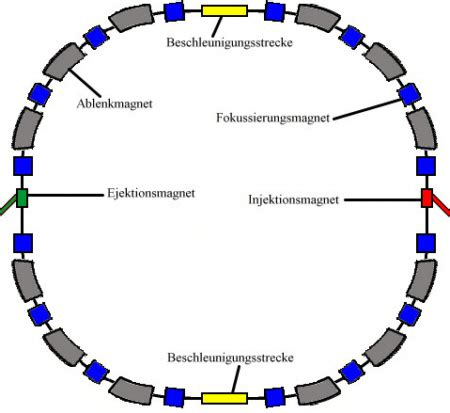
\includegraphics[width=1\linewidth]{figures/teilchenbe.jpg}
            \caption{Synchrotron}
            \label{fig:teilchenbe}
        \end{figure}
    \end{columns}
\end{frame}

\section{Wirkungsquerschnitt}
\begin{frame}{Wirkungsquerschnitt}
    \begin{columns}[c]
        \column{.45\textwidth}
        \begin{itemize}
            \item Maß für Wahrscheinlichkeit für Wechselwirkung
            \item Dimension einer Fläche
            \item Einheit Barn $1b = 10^{-28}cm^2$
            \item $w=\sigma \frac{N_T}{F}\quad. \implies \quad \sigma=w\frac{F}{N_T}$
        \end{itemize}

        \column{.45\textwidth}
        \begin{figure}
            \centering
            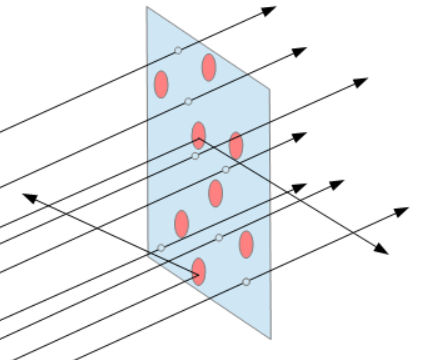
\includegraphics[width=1\linewidth]{figures/Wirkungsquerschnitt.png}
            \caption{Wirkungsquerschnitt}
            \label{fig:Wirkungsquerschnitt}
        \end{figure}
    \end{columns}
\end{frame}
\begin{frame}{Wirkungsquerschnitt}
    \begin{columns}[c]
        \column{.45\textwidth}
        \begin{itemize}
            \item Versuch am Petra Beschleuniger
            \item Elektron + Positron zu Myon Paar
            \item differentielle Wirkungsquerschnitt $\frac{d\sigma}{d\Omega}$
            \item Vergleich mit Standartmodell
        \end{itemize}

        \column{.45\textwidth}
        \begin{figure}
            \centering
            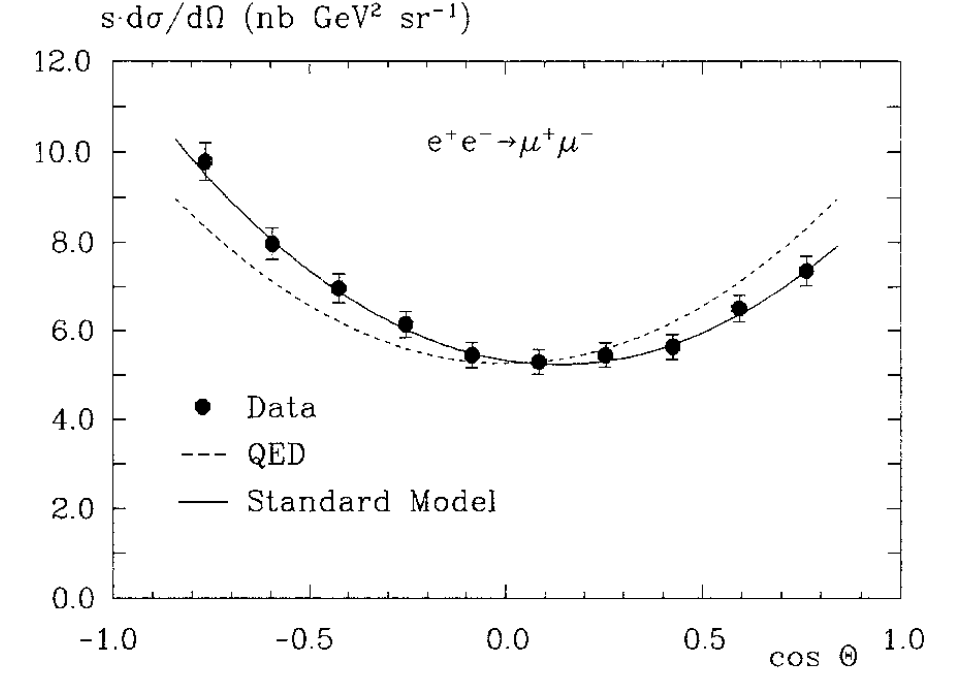
\includegraphics[width=1\linewidth]{figures/Petra.png}
            \caption{Daten Petra Beschleuniger}
            \label{fig:Petra}
        \end{figure}
    \end{columns}
\end{frame}

\section{Phasenraumintegration}
\begin{frame}{Phasenraum}
    \begin{block}{Definition}
        Der Phasenraum beschreibt alle möglichen Zustände eines physikalischen Systems
    \end{block}
    \vspace{10pt}
    \begin{columns}[c]
        \column{.3\textwidth}
        \textbf{Phasenraum in der Teilchenphysik} \\
        \begin{itemize}
            \item umfasst die Impulse \( \vec{p} \) und Energien \( E \) der beteiligten Teilchen
            \item Integration zur Berechung physikalischer Größen
        \end{itemize}
        \column{.65\textwidth}
        \pause
        \begin{exampleblock}{System von n Teilchen im Endzustand}
            \[
                d\Phi_n = \prod_{i=1}^n \frac{d^3p_i}{(2\pi)^3 2E_i} \cdot (2\pi)^4 \delta^4\left(p_{\text{initial}} - \sum_{i=1}^n p_i\right),
            \] \\
            \vspace{10pt}
            $d\Phi_n$: differentielles Phasenraumelement \\
            $p_i = (E_i, \overrightarrow{p}_i)$: Viererimplus des $i$-ten Teilches
        \end{exampleblock}
    \end{columns}
\end{frame}

\begin{frame}{Phasenraum: Beispiel}
    \begin{figure}
        \centering
        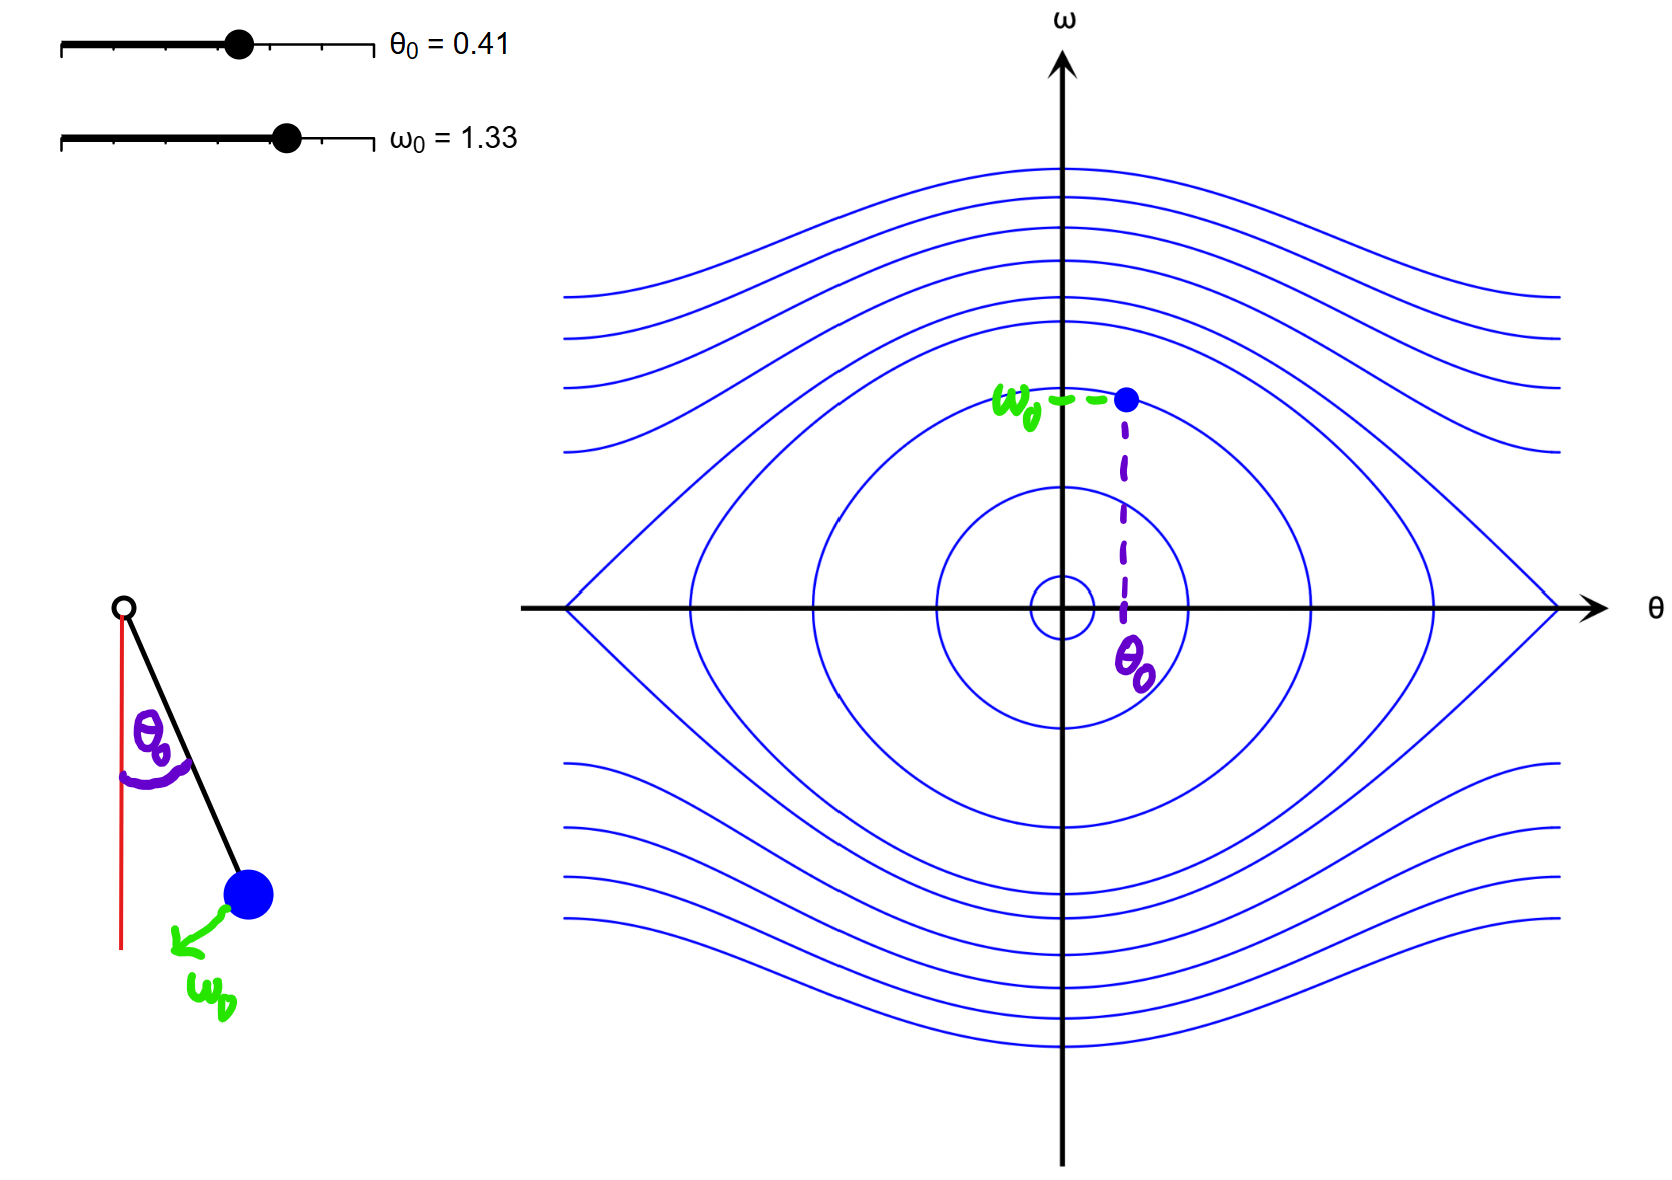
\includegraphics[width=0.55\linewidth]{figures/phasespace.png}
        \caption{Phasenraum eines Fadenpendels ohne Energieverluste}
        \label{fig:phasespace}
    \end{figure}
\end{frame}

\begin{frame}{Phasenraumintegration}
    \begin{columns}[c]
        \column{.45\textwidth}
        Integration über den Viererimpuls $p_i = (E_i, \overrightarrow{p}_i)$ von $n$ Teilchen
        \vspace{10pt}
        \begin{block}{Verwendung}
            \textbf{Berechnung physikalischer Größen}
            \begin{itemize}
                \item Wirkungsquerschnitte (\( \sigma \)) für Streuprozesse
                \item Zerfallsraten (\( \Gamma \)) für Teilchenzerfälle
            \end{itemize}
        \end{block}
        \column{.45\textwidth}
        \begin{exampleblock}{Methoden}
            \textbf{Analytische Integration}
            \begin{itemize}
                \item für einfache Prozesse
                \item z.B. Zwei-Teilchen-Zerfall
            \end{itemize}
            \vspace{10pt}
            \textbf{Numerische Methoden}
            \begin{itemize}
                \item für komplexe Prozesse
                \item mit mehreren Endzustandsteilchen
                \item z.B. mit Monte-Carlo-Integration
            \end{itemize}
        \end{exampleblock}
    \end{columns}
\end{frame}

\begin{frame}{Monte-Carlo Methode}
    \begin{columns}[c]
        \column{.5\textwidth}
        \begin{exampleblock}{Beispiel: Nährung von $\pi$}
            \begin{enumerate}
                \item Generation zufälliger Punkte \( (x, y) \) in einem Quadrat mit Seitenlänge 1
                \item Prüfe, ob der Punkt innerhalb des Viertelkreises liegt: \( x^2 + y^2 \leq 1 \).
                \item Verhältnis der Punkte im Kreis zu allen generierten Punkten entspricht \( \pi/4 \).
            \end{enumerate}
        \end{exampleblock}
        \column{.45\textwidth}
        \begin{figure}
            \centering
            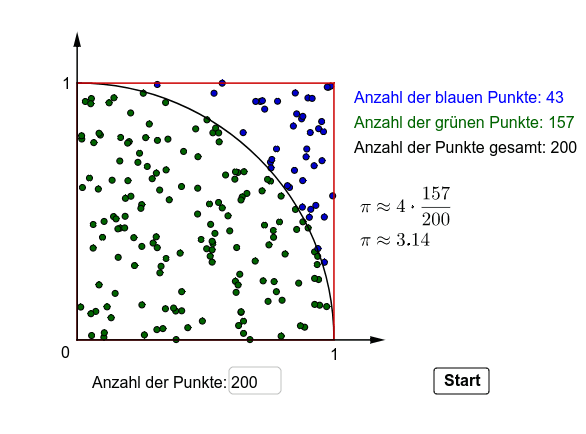
\includegraphics[width=0.9\linewidth]{figures/montecarlo.png}
            %\caption{Monte-Carlo-Methode}
            \label{fig:montecarlo}
        \end{figure}
    \end{columns}
    \pause
    \begin{alertblock}{Übertragung auf die Teilchenphysik}
        \begin{itemize}
            \item Integration über den Phasenraum mit zufälligen Proben
            \item $\implies$ effizientes Lösen von Mehrteilchen-Endzuständen
        \end{itemize}
    \end{alertblock}
\end{frame}

\begin{frame}{Heutige Forschung}
    \begin{columns}[c]
        \column{.45\textwidth}
        \begin{block}{Myon-G-2 Experiment}
            \begin{itemize}
                \item Messung des anomalen magnetischen Moments des Myons
                \item Abweichung vom Standardmodell
                \item Hinweis auf neue Physik
            \end{itemize}
        \end{block}
        \column{.45\textwidth}
        \begin{figure}
            \centering
            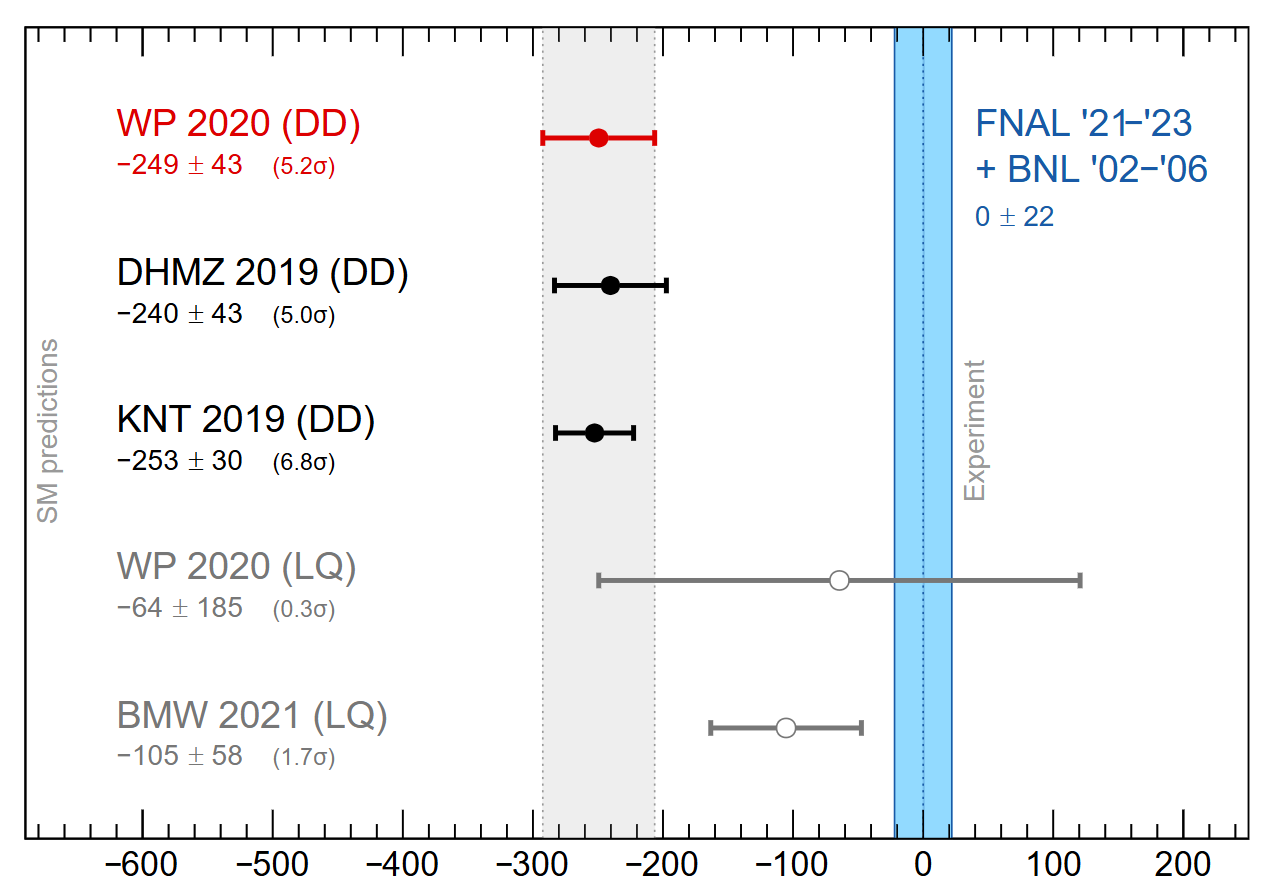
\includegraphics[width=0.9\linewidth]{figures/myonmagn.png}
            \caption{Myon magnetisches Moment}
            \label{fig:myonmagn}
        \end{figure}
    \end{columns}
\end{frame}

\begin{frame}[allowframebreaks]{Literaturverzeichnis}
    \nocite{*}
    \footnotesize
    \bibliography{reference.bib}
    \bibliographystyle{apalike}
\end{frame}

\end{document}

\section{Phasenraumintegration}
\begin{frame}{Phasenraum}
    % was ist ein Phasenraum überhaupt
\end{frame}

\begin{frame}{Phasenraumintegration}
    % Notwendigkeit?, Methoden?
\end{frame}

\begin{frame}{Monte-Carlo Methode}
    % am Beispiel erklären mit \pi
\end{frame}

%------------------------------------------------
\section{First Section}
%------------------------------------------------

\begin{frame}{Bullet Points}
    \begin{itemize}
        \item Lorem ipsum dolor sit amet, consectetur adipiscing elit
        \item Aliquam blandit faucibus nisi, sit amet dapibus enim tempus eu
        \item Nulla commodo, erat quis gravida posuere, elit lacus lobortis est, quis porttitor odio mauris at libero
        \item Nam cursus est eget velit posuere pellentesque
        \item Vestibulum faucibus velit a augue condimentum quis convallis nulla gravida
    \end{itemize}
\end{frame}

%------------------------------------------------

\begin{frame}{Blocks of Highlighted Text}
    In this slide, some important text will be \alert{highlighted} because it's important. Please, don't abuse it.

    \begin{block}{Block}
        Sample text
    \end{block}

    \begin{alertblock}{Alertblock}
        Sample text in red box
    \end{alertblock}

    \begin{examples}
        Sample text in green box. The title of the block is ``Examples".
    \end{examples}
\end{frame}

%------------------------------------------------


\begin{columns}[c]
    \column{.45\textwidth}
    \column{.45\textwidth}
\end{columns}

\begin{frame}{Multiple Columns}
    \begin{columns}[c] % The "c" option specifies centered vertical alignment while the "t" option is used for top vertical alignment

        \column{.45\textwidth} % Left column and width
        \textbf{Heading}
        \begin{enumerate}
            \item Statement
            \item Explanation
            \item Example
        \end{enumerate}

        \column{.45\textwidth} % Right column and width
        Lorem ipsum dolor sit amet, consectetur adipiscing elit. Integer lectus nisl, ultricies in feugiat rutrum, porttitor sit amet augue. Aliquam ut tortor mauris. Sed volutpat ante purus, quis accumsan dolor.

    \end{columns}
\end{frame}

%------------------------------------------------
\section{Second Section}
%------------------------------------------------

\begin{frame}{Table}
    \begin{table}
        \begin{tabular}{l l l}
            \toprule
            \textbf{Treatments} & \textbf{Response 1} & \textbf{Response 2} \\
            \midrule
            Treatment 1         & 0.0003262           & 0.562               \\
            Treatment 2         & 0.0015681           & 0.910               \\
            Treatment 3         & 0.0009271           & 0.296               \\
            \bottomrule
        \end{tabular}
        \caption{Table caption}
    \end{table}
\end{frame}

%------------------------------------------------

\begin{frame}{Theorem}
    \begin{theorem}[Mass--energy equivalence]
        $E = mc^2$
    \end{theorem}
\end{frame}

%------------------------------------------------

\begin{frame}{Figure}
    Uncomment the code on this slide to include your own image from the same directory as the template .TeX file.
    \begin{figure}
        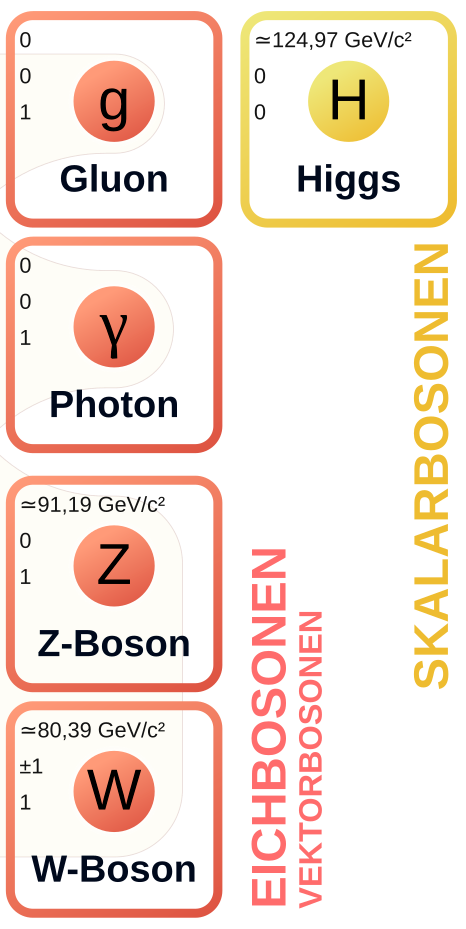
\includegraphics[height=0.15\paperheight]{figures/bosonen.png}
        \caption{Test Bosonen}
        \label{fig:bosonen}
    \end{figure}
\end{frame}

%------------------------------------------------

\begin{frame}[fragile] % Need to use the fragile option when verbatim is used in the slide
    \frametitle{Citation}
    An example of the \verb|\cite| command to cite within the presentation:\\~

    This statement requires citation \cite{p1}.
\end{frame}